\documentclass[]{article}

% Imported Packages
%------------------------------------------------------------------------------
\usepackage{amssymb}
\usepackage{amstext}
\usepackage{amsthm}
\usepackage{amsmath}
\usepackage{enumerate}
\usepackage{fancyhdr}
\usepackage{float} %the picture keeps floating away from where it's supposed to
\usepackage[margin=1in]{geometry}
\usepackage{graphicx}
\usepackage{hyperref}
\usepackage{extarrows}
\usepackage{setspace}
%------------------------------------------------------------------------------

% Header and Footer
%------------------------------------------------------------------------------
\pagestyle{plain}  
\renewcommand\headrulewidth{0.4pt}                                      
\renewcommand\footrulewidth{0.4pt}                                    

\hypersetup{            % sets colours for hyperlinks
    colorlinks=true,    % false: boxed links; true: colored links
    linkcolor=blue,     % colour of internal links (change box color with linkbordercolor)
    citecolor=black,    % colour of links to bibliography
	filecolor=black,    % colour of file links
	urlcolor=black      % colour of external links
}
%------------------------------------------------------------------------------

% Title Details
%------------------------------------------------------------------------------
    \newcommand{\thetitle}{Cabshare - Deliverable 3} % for making the pdf produced have professional naming
\title{\thetitle}
%\author{SE 3A04: Software Design II -- Large System Design}
\date{\today}                               
%------------------------------------------------------------------------------

% Author
\author{	Ahmed, Kemal\\
	\and
	Bhutta, Sahajmeet\\
	\and
	Spector, Mitchell\\
	\and
	Xiao, Yuchen\\
	\and
	Lin, Xue\\
}

\usepackage{fancyhdr}
\pagestyle{fancy}
\makeatletter
\makeatother

%allow for diagram stuff
\usepackage{tikz}
\usepackage{verbatim}

% Document
%------------------------------------------------------------------------------
\begin{document}

\begin{titlepage}
\begin{center}


\textsc{\LARGE McMaster University}\\[1.5cm]

\textsc{\Large SFWR ENG 3A04: T1-05}\\[0.5cm]

% Title


{ \huge \textbf{\textsc{\thetitle}}\\[0.4cm] }

\vfill

% Author and supervisor
\begin{flushleft} \large

\newcommand{\itab}[1]{\hspace{0em}\rlap{#1}}
\newcommand{\tab}[1]{\hspace{.2\textwidth}\rlap{#1}}

\emph{Authors:}\\
\itab{Kemal \textsc{Ahmed}}  \tab{}  \tab{\emph{ahmedks}}  \tab{}  \tab{1150377}\\
\itab{Mitchell \textsc{Spector}}    \tab{}  \tab{\emph{spectoriscool}} \tab{}  \tab{1208006}\\
\itab{Sahajmeet \textsc{Bhutta}}    \tab{}  \tab{\emph{bhuttas}}   \tab{}  \tab{1223708}\\
\itab{Xue \textsc{Lin}} \tab{}  \tab{\emph{liniscool}}  \tab{}  \tab{1151043}\\
\itab{Yuchen \textsc{Xiao}} \tab{}  \tab{\emph{xiaoy23}}   \tab{}  \tab{1212583}


\end{flushleft}

\vfill

% Bottom of the page
{\large \today}
\end{center}
\end{titlepage}

\tableofcontents
\newpage

\section{Introduction}
\label{sec:introduction}
% Begin Section

\subsection{Purpose}
\label{sub:purpose}
% Begin SubSection
	 This document is intended to formalize the classes which will be used in the final application. It depicts states of controller classes, how use cases unfold through sequence diagrams, and attributes and methods of classes. Its intended audience is the development team and software engineers.
% End SubSection

\subsection{System Description}
\label{sub:system_description}

The system is designed to securely allow users to search for cabs with passengers willing to cabpool to a user’s destination, or include a stop along the way to a further destination, and to allow users to offer a cab for cabpooling. The system will connect commuters and cabpoolers to lower individual fares while still providing a profit for the cab company.
\subsection{Overview}
\label{sub:overview}
% Begin SubSection
	This document consists almost entirely of diagrams, including state charts, sequence diagrams, and a class diagram, respectively. State charts depict the various states induced in each controller class, sequence diagrams depict messages and data passed between classes as use cases are occuring, and the class diagram depics communication between classes.
% End SubSection


% Begin Section
\section{State Charts for Controller Classes}
\label{sec:state_charts_for_controller_classes}

\subsection{CancelController}
\begin{figure}[H]
\label{CCState}
	\centering
	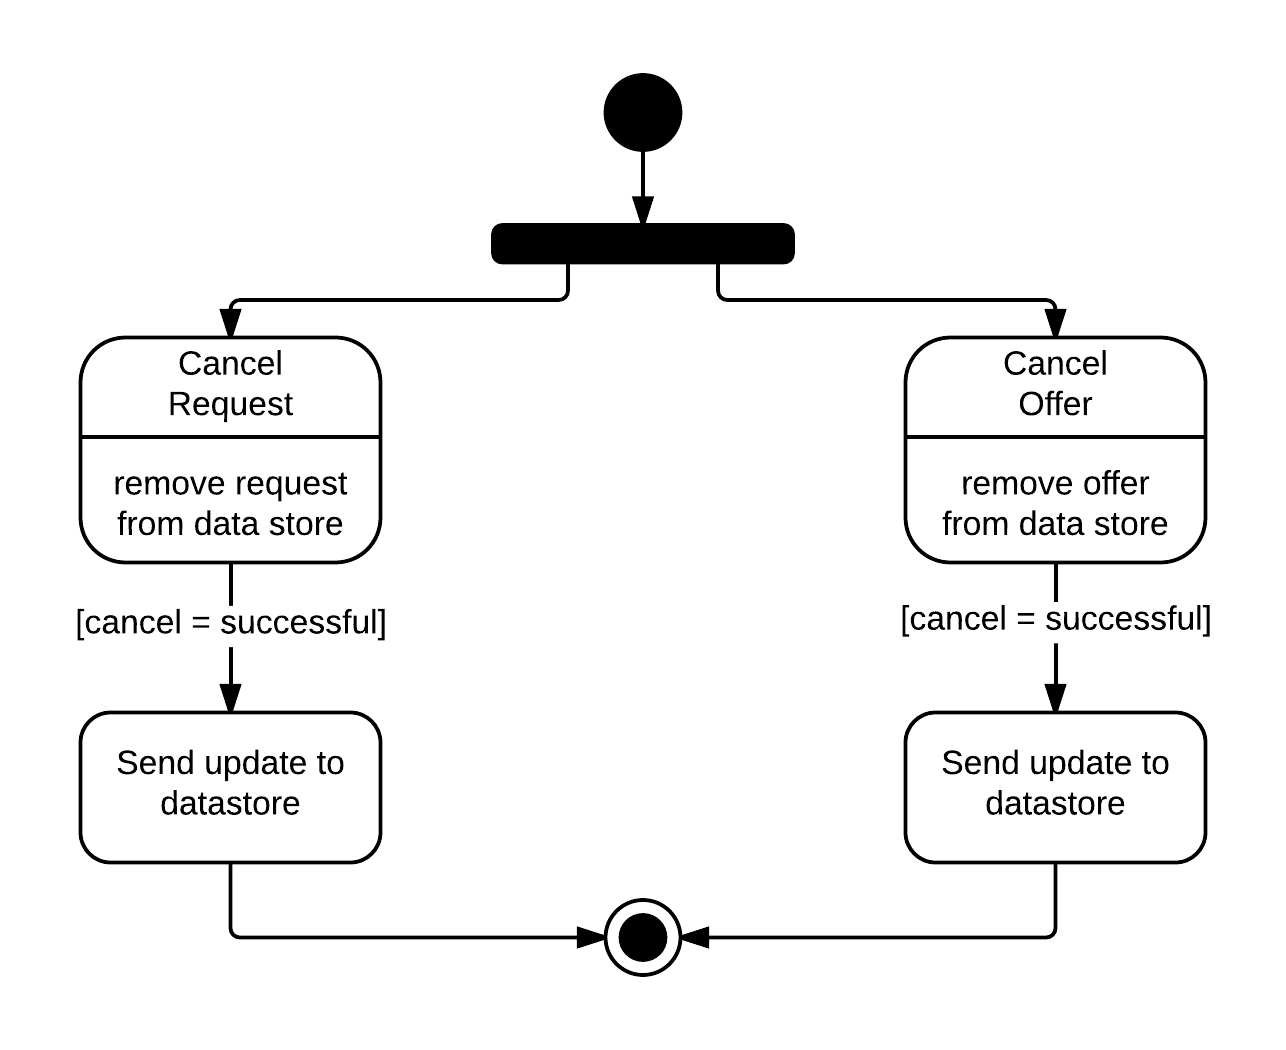
\includegraphics[width=1\textwidth]{CancelController.png}
	\caption{\textbf{State Diagram of CancelController} When user wants to cancel their request to join a cabpool.}
\end{figure}
% End Subsection

\subsection{Encryptor}
\begin{figure}[H]
\label{encrypt}
	\centering
	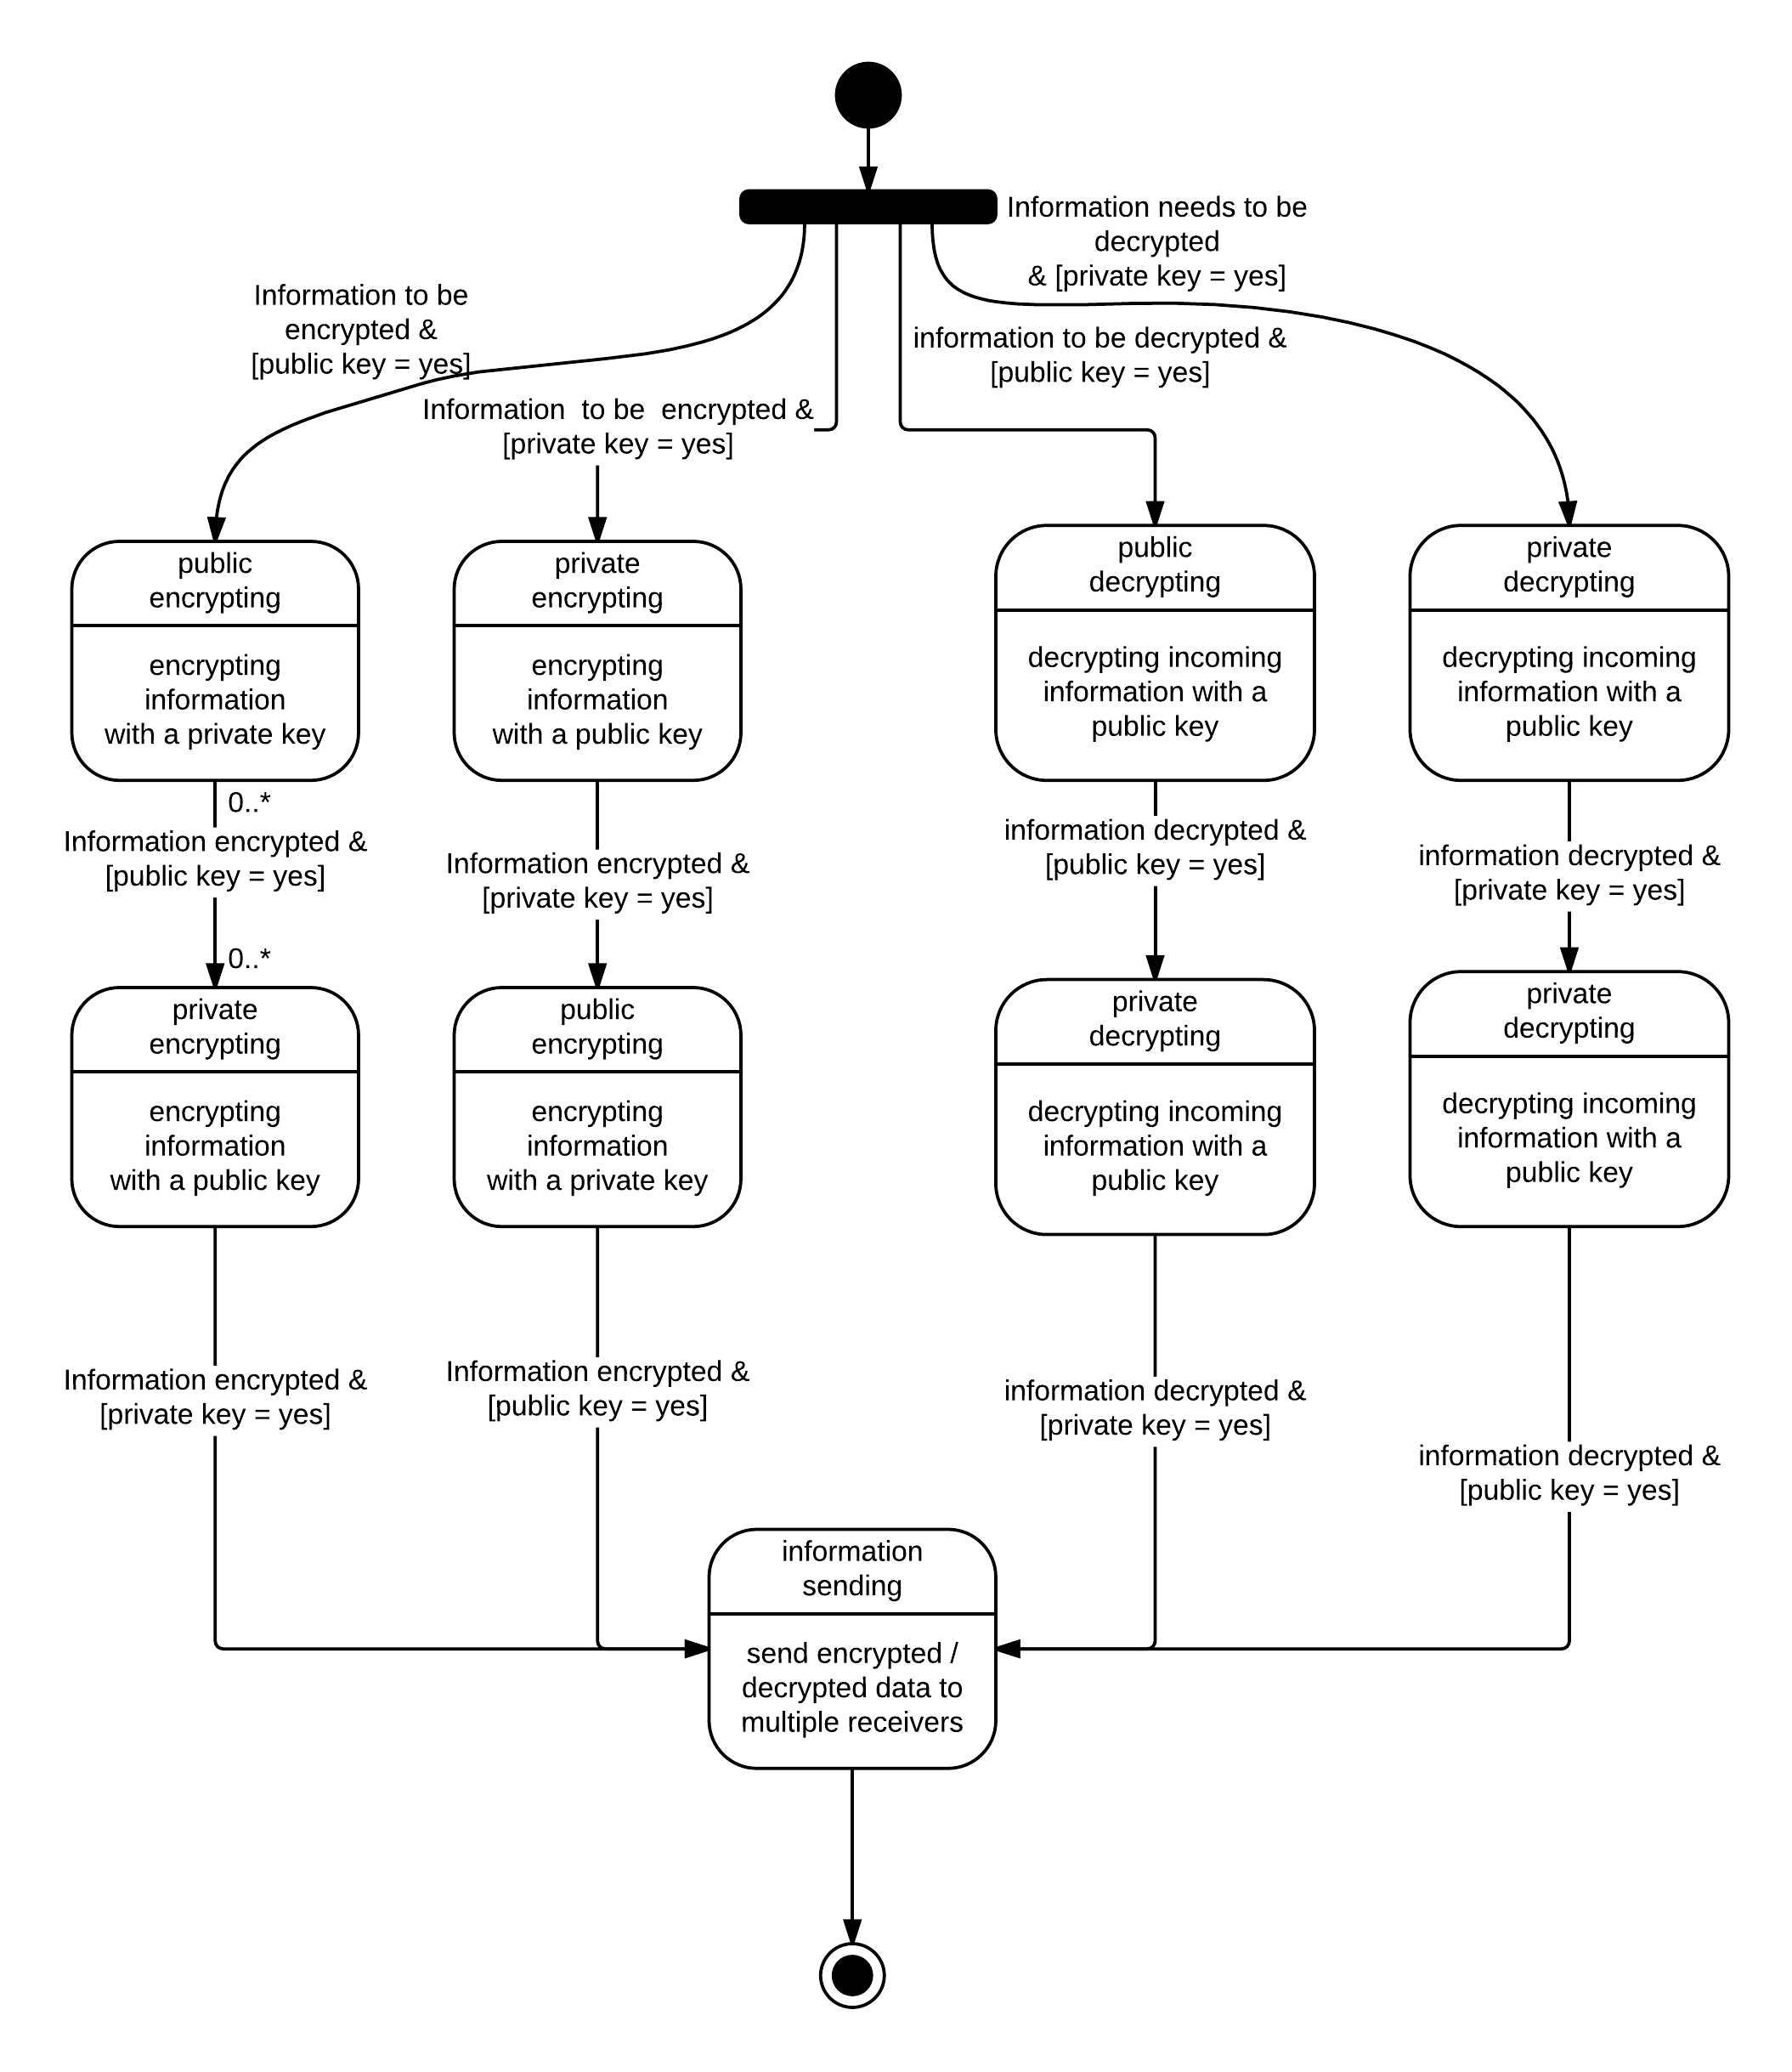
\includegraphics[width=1\textwidth]{Encryptor.png}
	\caption{\textbf{State Diagram of Encryptor} Encrypting messages between people waiting for their ride and the people already in the cabpool.}
\end{figure}
% End Subsection

\subsection{LogoutController}
\begin{figure}[H]
\label{LCState}
	\centering
	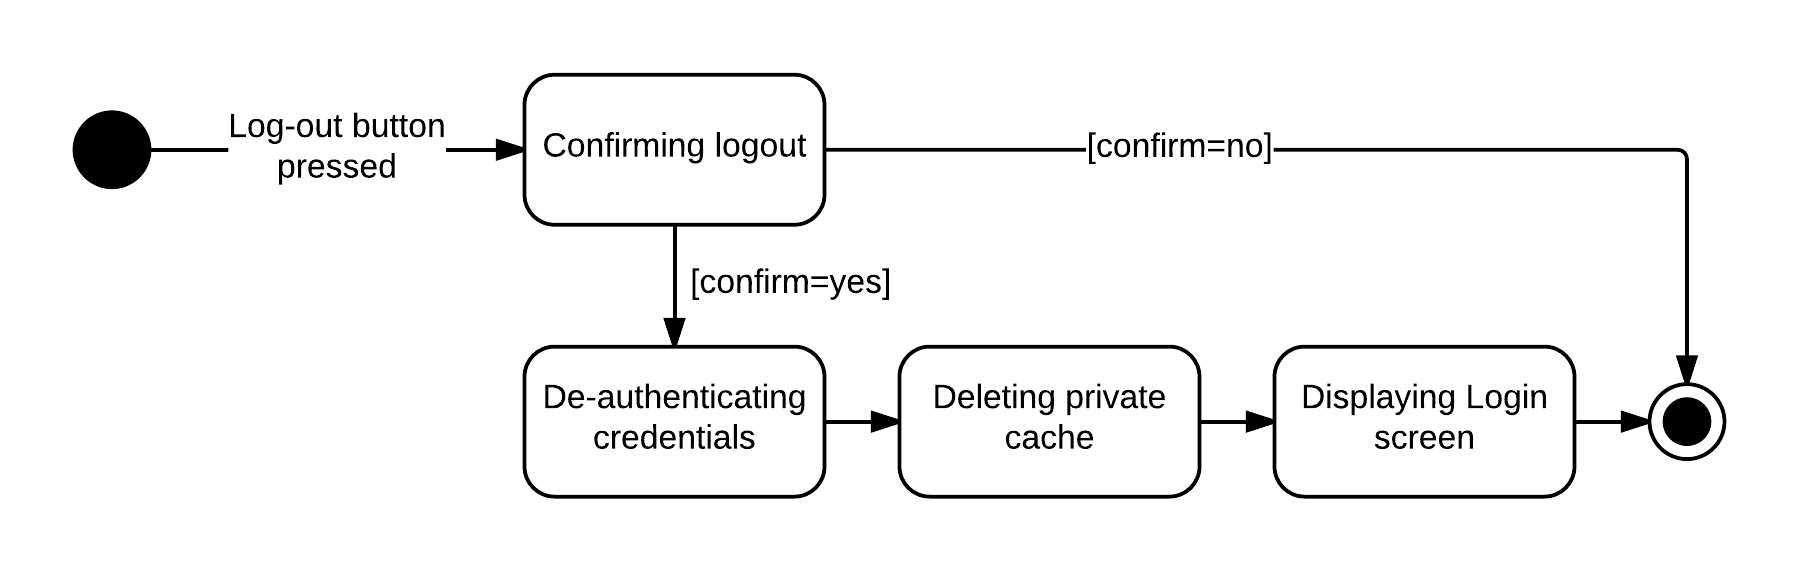
\includegraphics[width=1\textwidth]{LogoutController.png}
	\caption{\textbf{State Diagram of LogoutController} When a user is logging out.}
\end{figure}
% End Subsection

\subsection{PaymentController}

\begin{figure}[H]
\label{PCState}
	\centering
	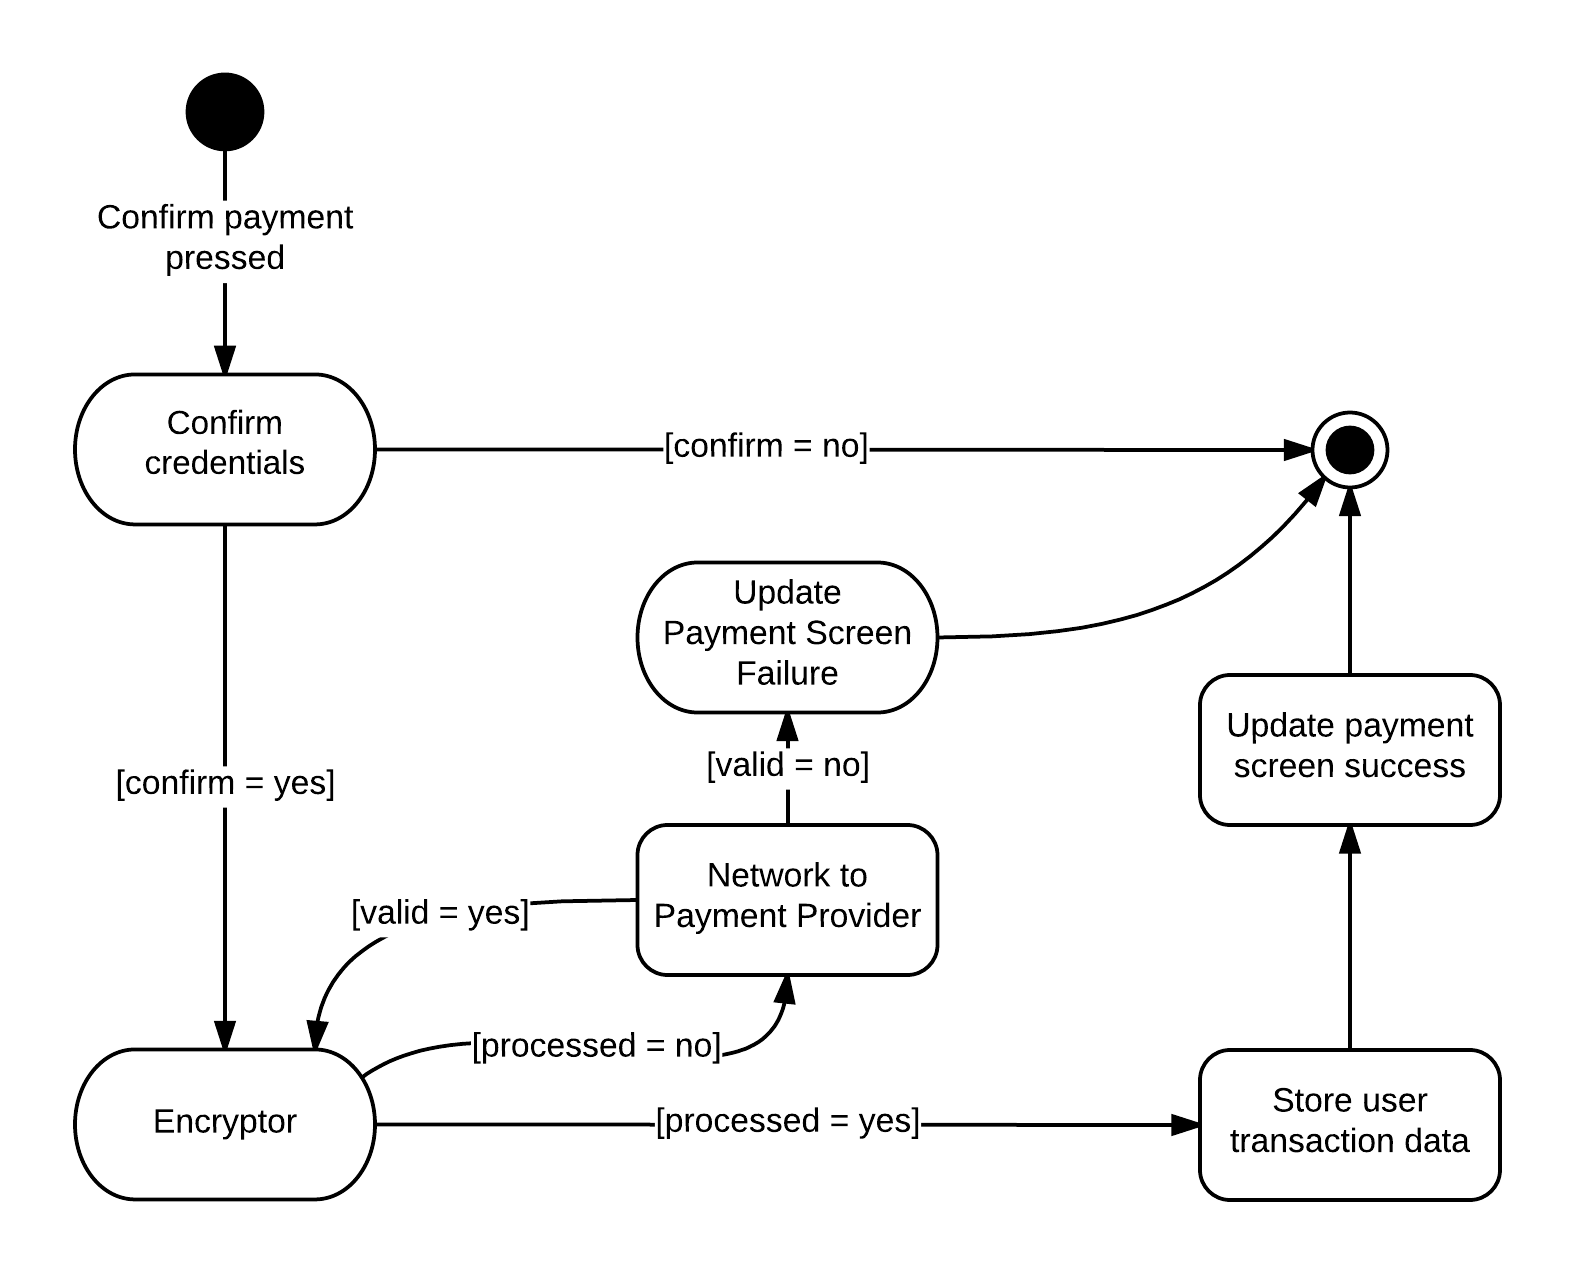
\includegraphics[width=1\textwidth]{PaymentController.png}
	\caption{\textbf{State Diagram of PaymentController} When a user is paying for their ride.}
\end{figure}
% End Subsection

\subsection{RoutesController}

\begin{figure}[H]
\label{RCState}
	\centering
	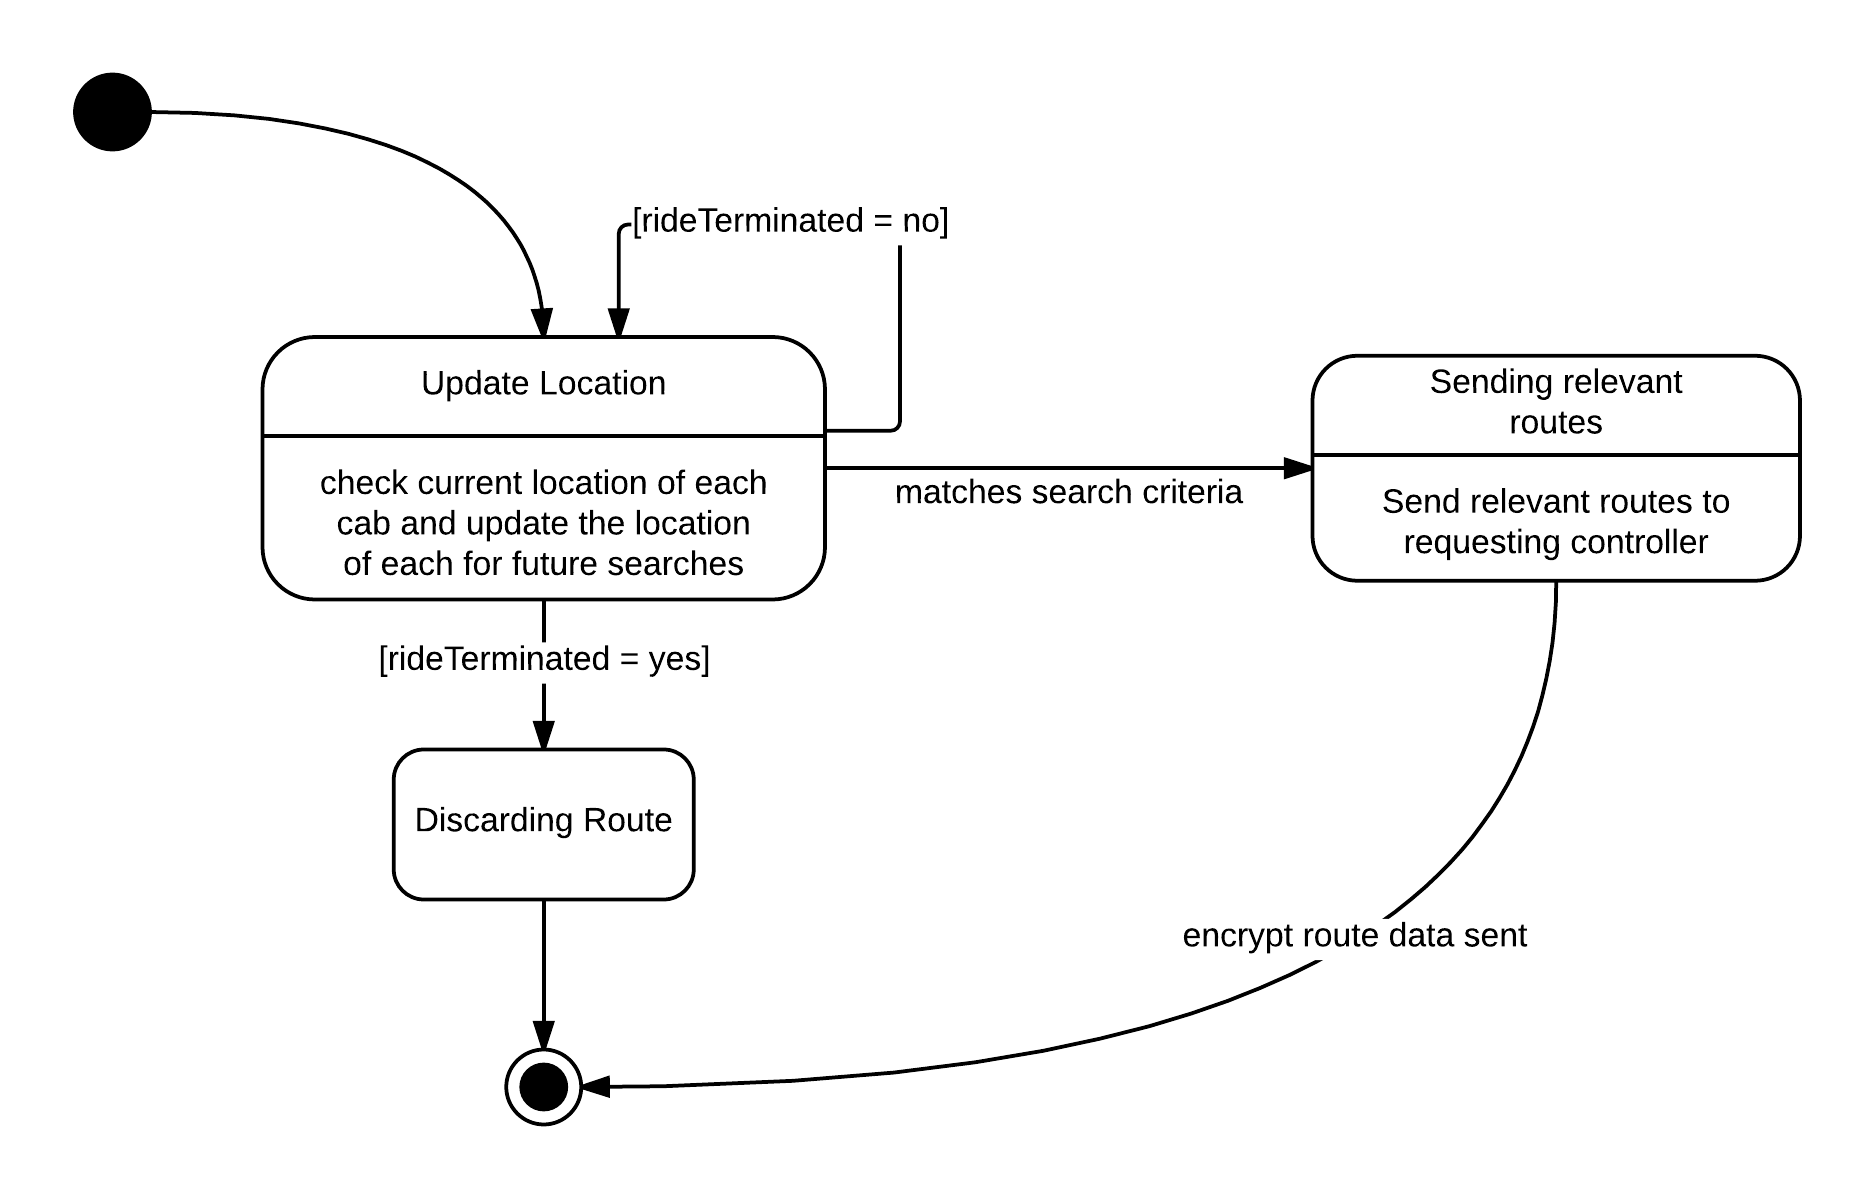
\includegraphics[width=1\textwidth]{RoutesController.png}
	\caption{\textbf{State Diagram of RoutesController} When a user is determining potential routes to their destination.}
\end{figure}
% End Subsection

\subsection{ScanController}

\begin{figure}[H]
\label{SCState}
	\centering
	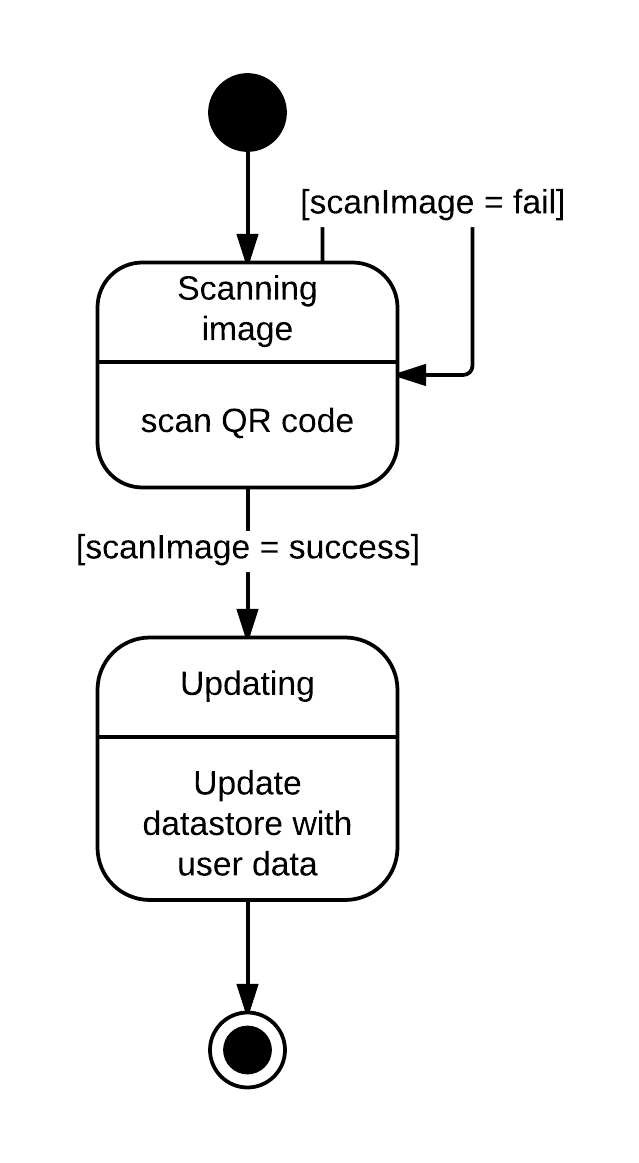
\includegraphics[height=0.5\textheight]{ScanController.png}
	\caption{\textbf{State Diagram of ScanController} When the user enters the cab and scans the QR code.}
\end{figure}
% End Subsection

\subsection{SecurityController}

\begin{figure}[H]
\label{SecCState}
	\centering
	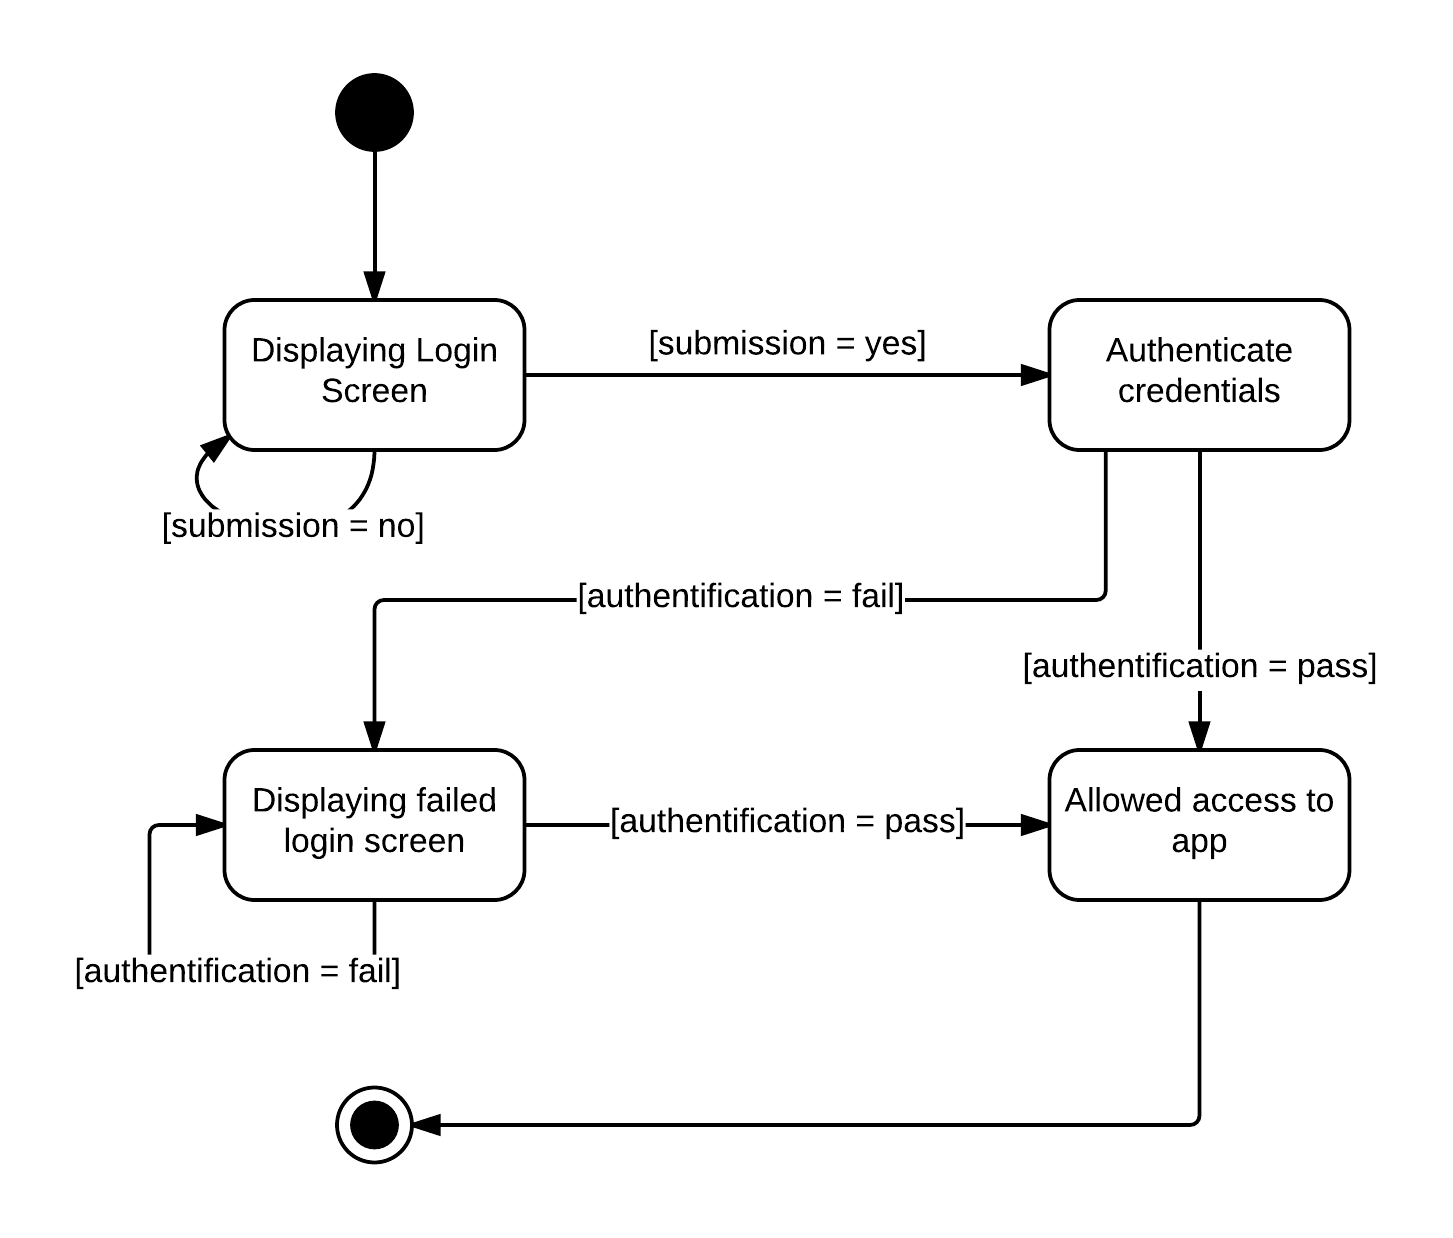
\includegraphics[width=1\textwidth]{SecurityController.png}
	\caption{\textbf{State Diagram of SecurityController} When the user is attempting to login.}
\end{figure}
% End Subsection

\subsection{SelectController}

\begin{figure}[H]
\label{SelCState}
	\centering
	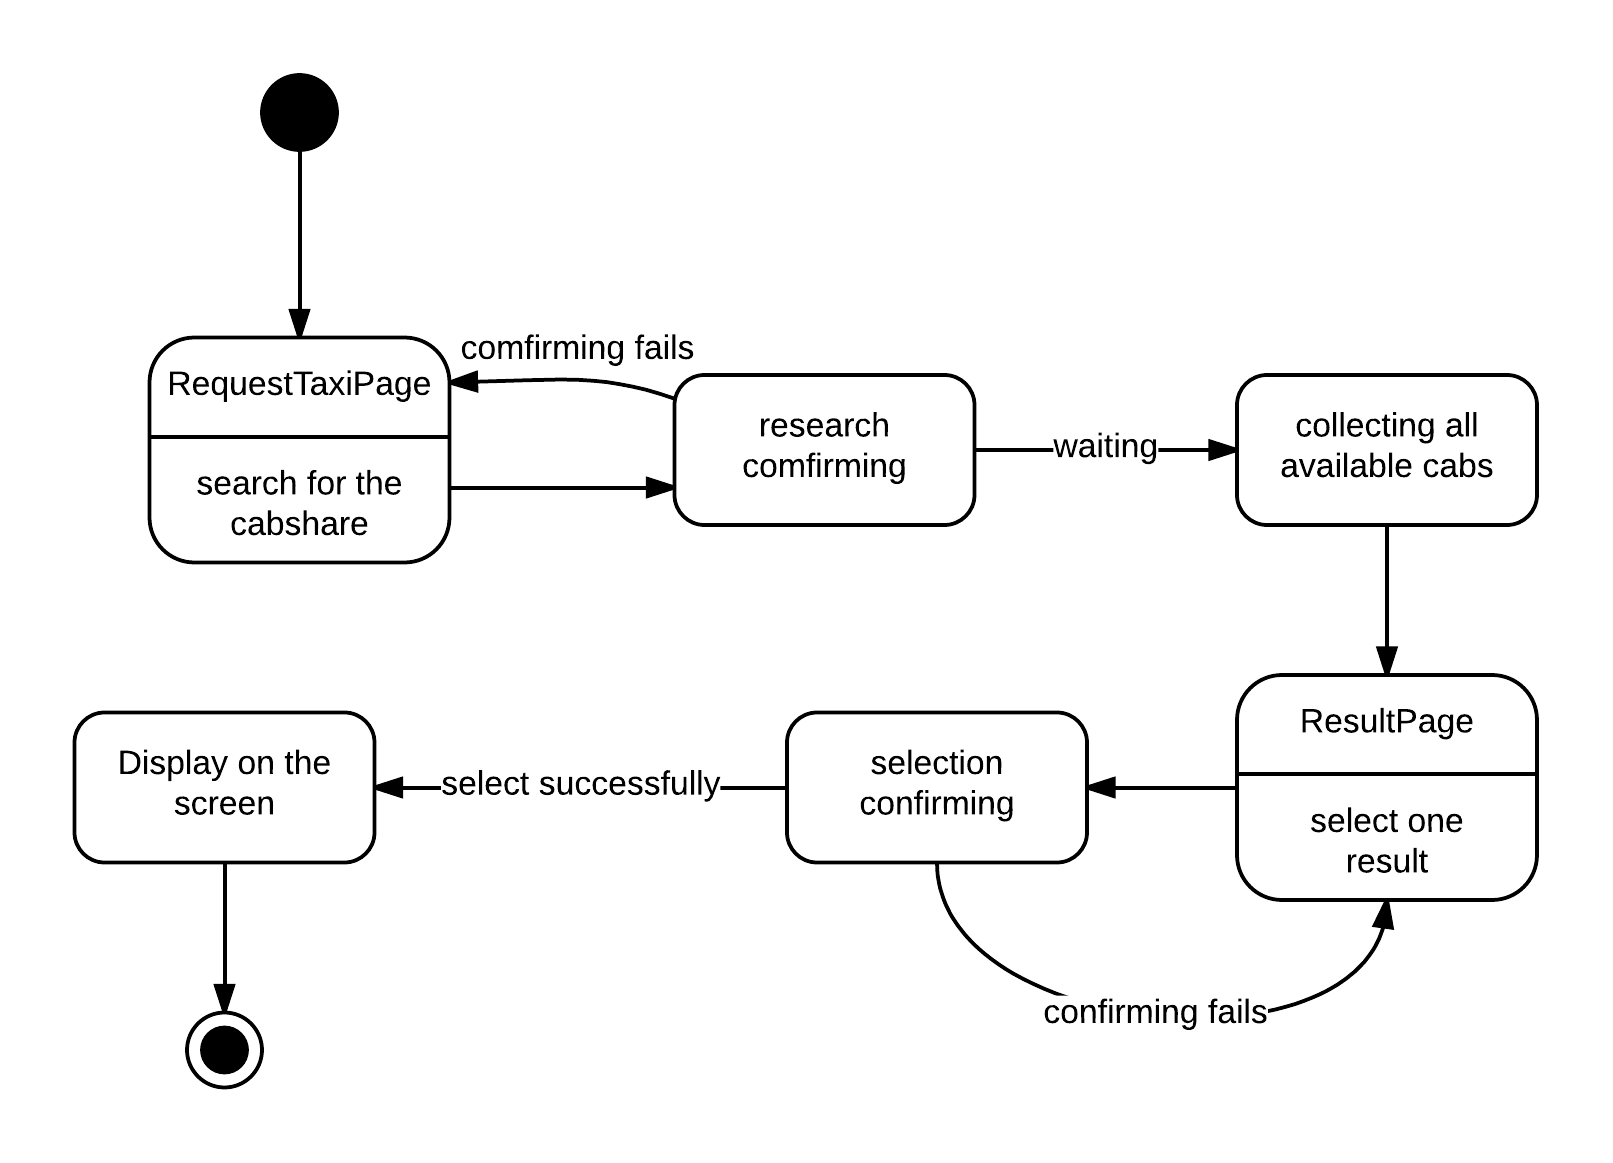
\includegraphics[width=1\textwidth]{SelectController.png}
	\caption{\textbf{State Diagram of SelectController} When user selects a cabpool to join.}
\end{figure}
% End Subsection

\subsection{ServerController}

\begin{figure}[H]
\label{SrvCState}
	\centering
	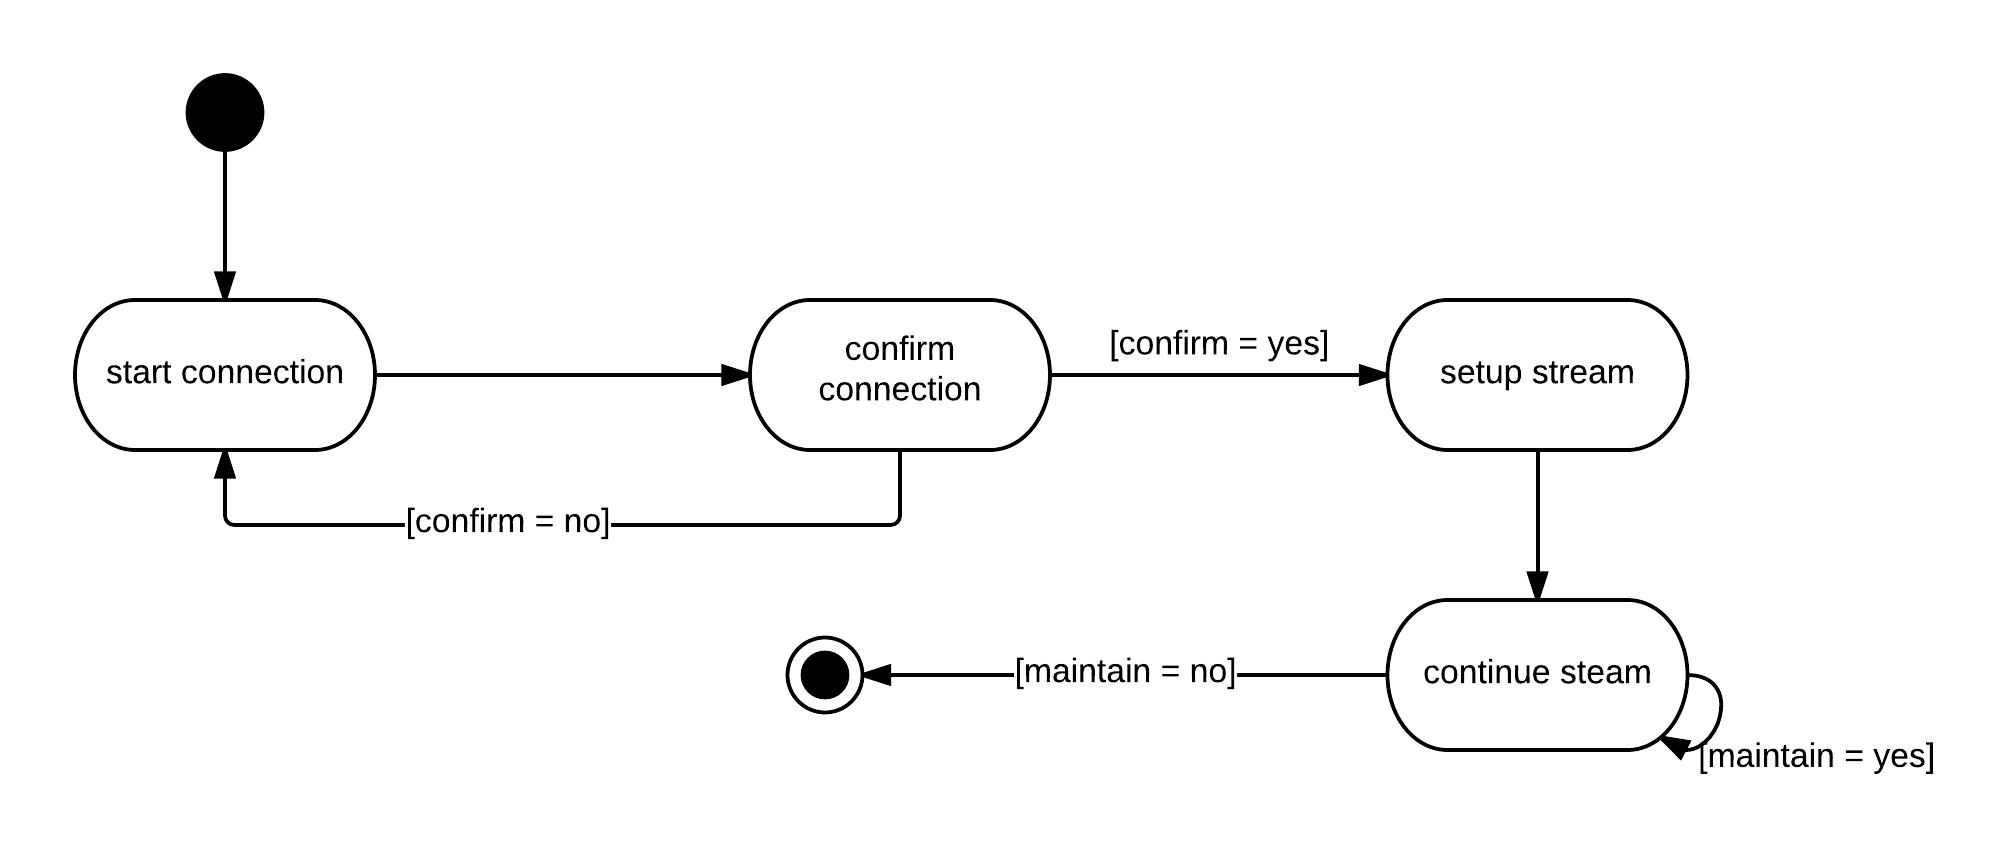
\includegraphics[width=1\textwidth]{ServerController.png}
	\caption{\textbf{State Diagram of ServerController} When the user tries to connect to the server initially.}
\end{figure}
% End Subsection

\subsection{TalkController}

\begin{figure}[H]
\label{TCState}
	\centering
	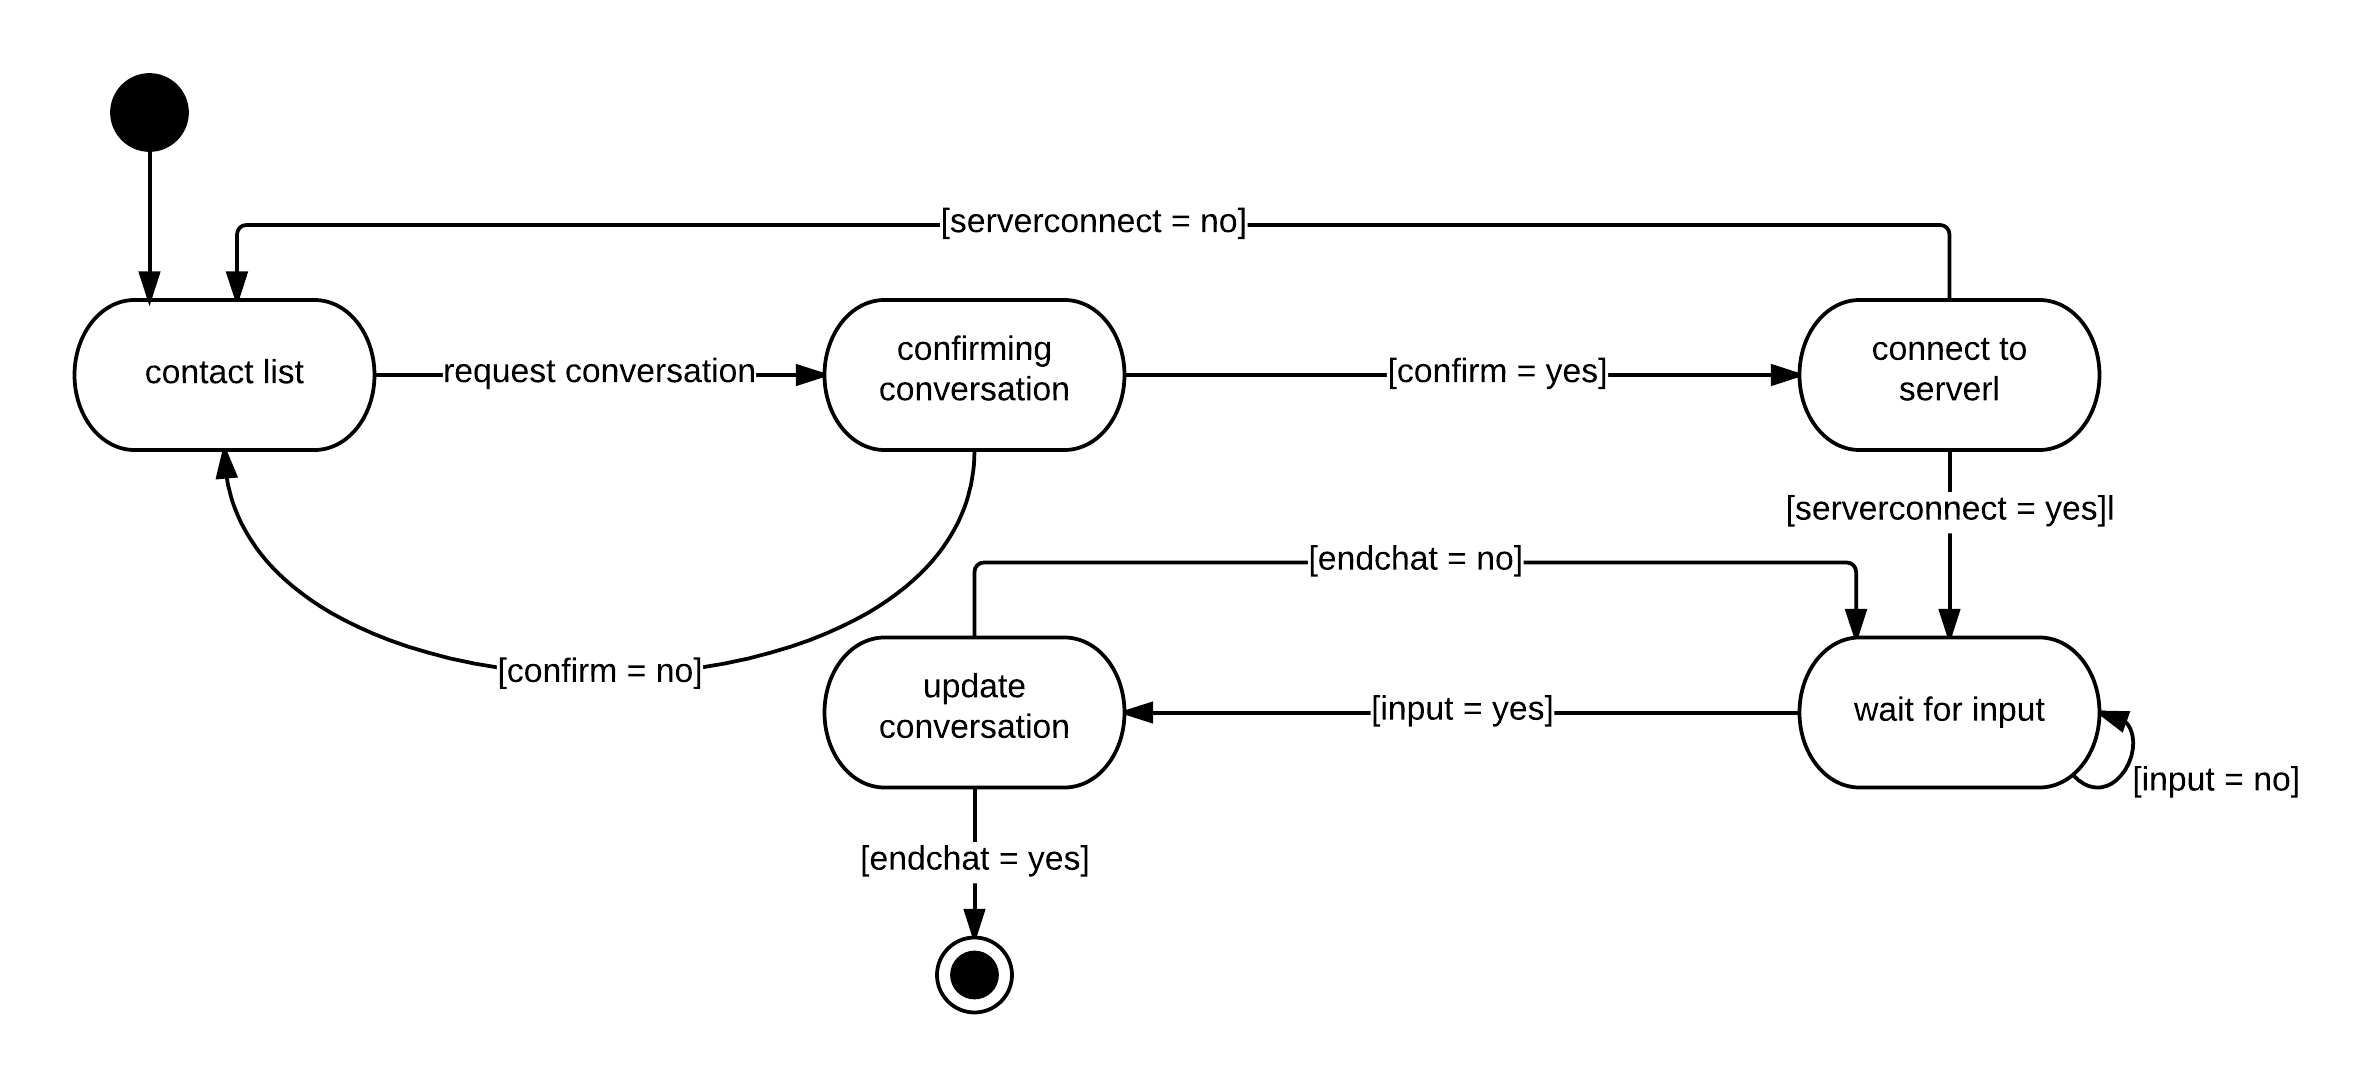
\includegraphics[width=1\textwidth]{TalkController.png}
	\caption{\textbf{State Diagram of TalkController} When the user wants to talk to the other people within the cabpool they are joining or when someone in the cabpool is communicating with someone they're going to pick up.}
\end{figure}
% End Subsection

\subsection{UserProfileController}

\begin{figure}[H]
\label{UPCState}
	\centering
	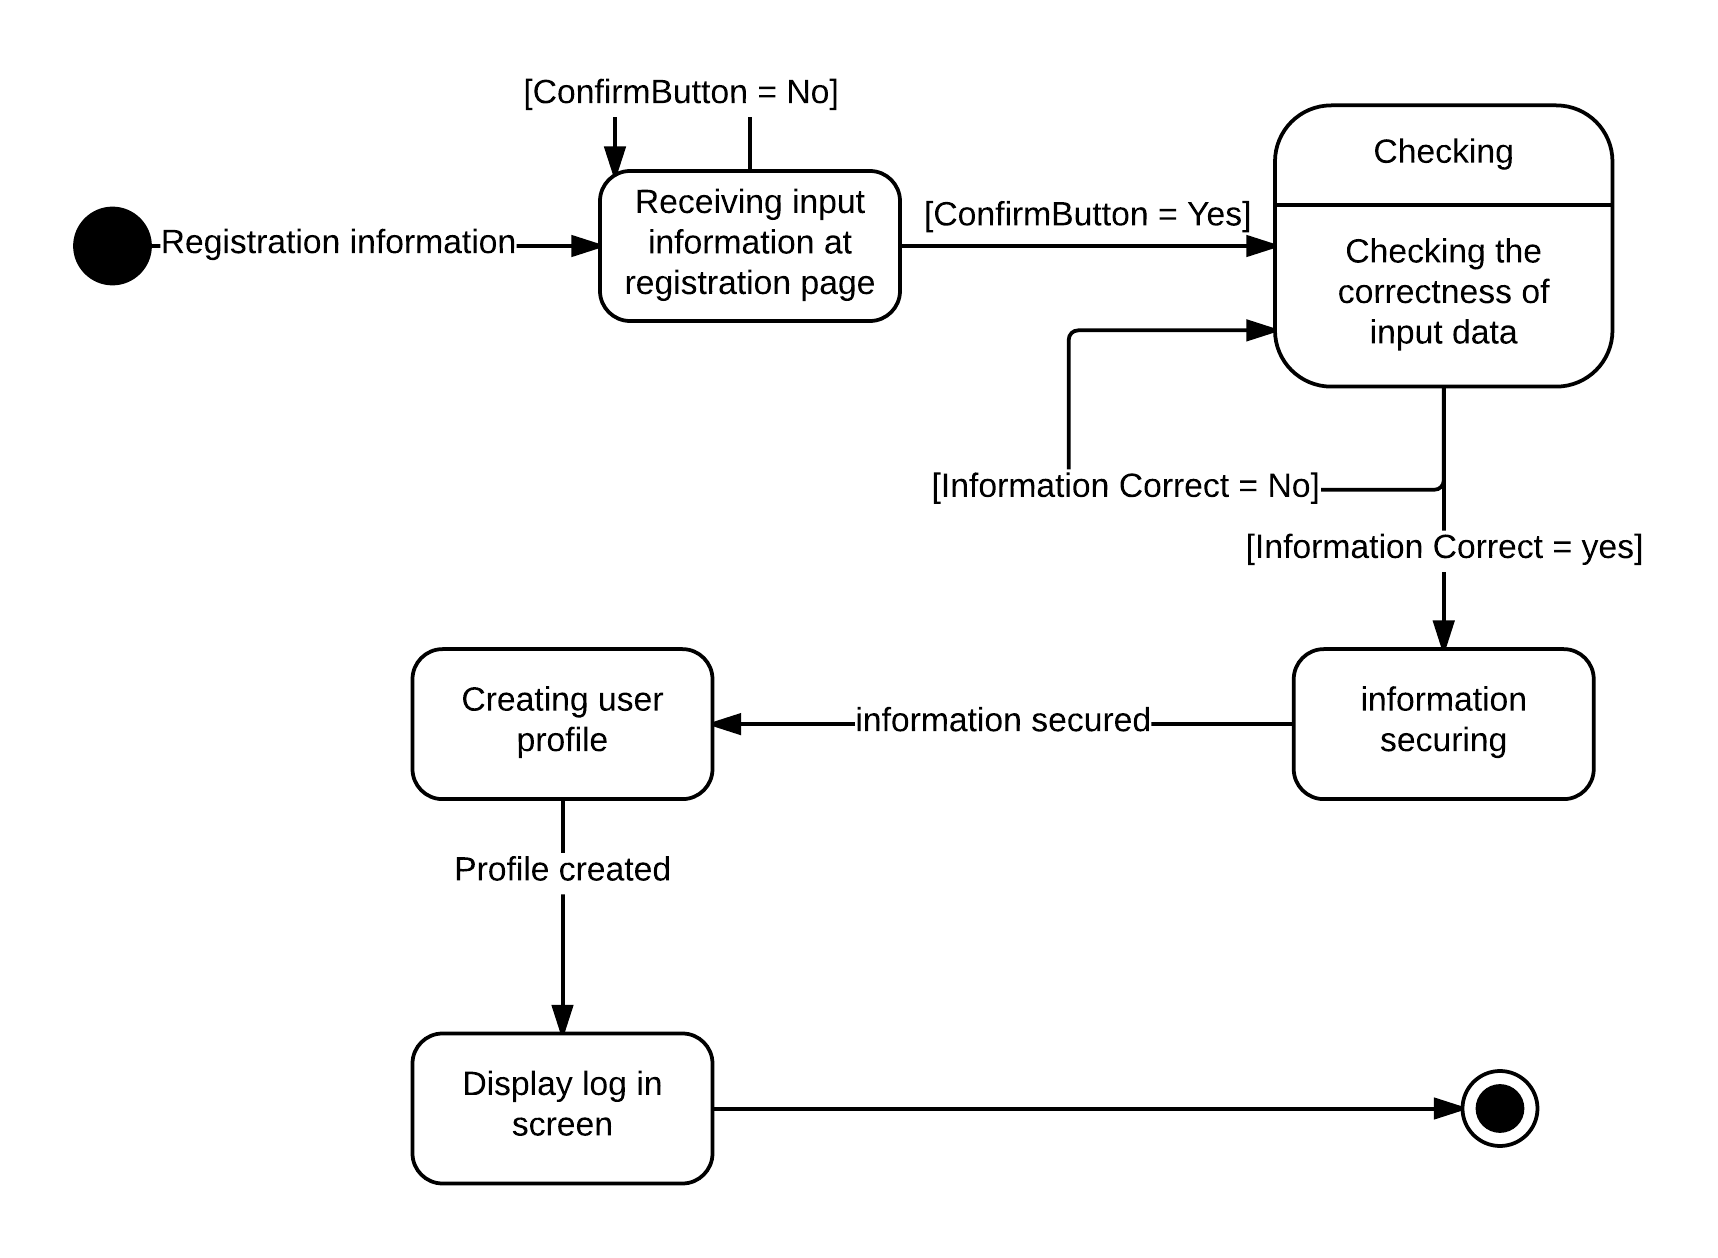
\includegraphics[width=1\textwidth]{UserProfileController.png}
	\caption{\textbf{State Diagram of UserProfileController} When the user first creates a profile.}
\end{figure}
% End Subsection

\subsection{UserRatingController}

\begin{figure}[H]
\label{URCState}
	\centering
	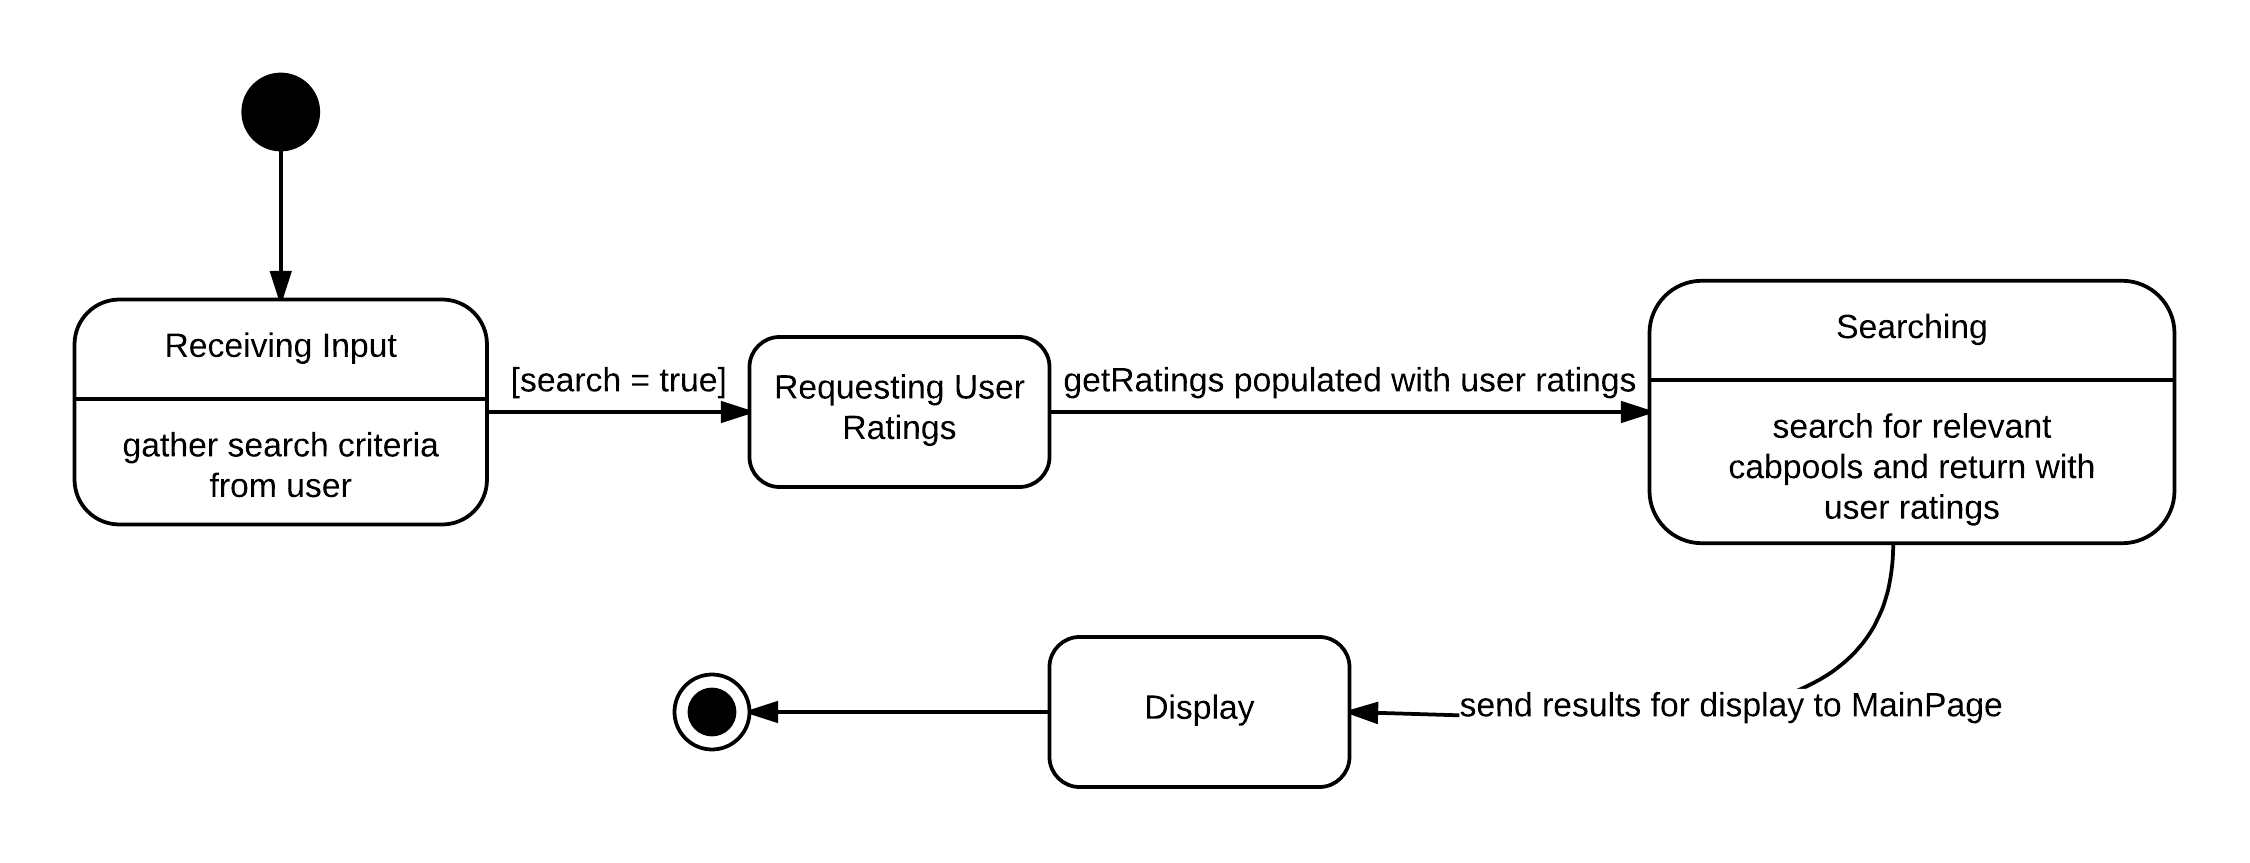
\includegraphics[width=1\textwidth]{UserRatingController.png}
	\caption{\textbf{State Diagram of UserRatingController} When a user wants to see the ratings of the user they're going to share the cabpool with.}
\end{figure}
% End Subsection
% End Section


% Begin Section
\section{Sequence Diagrams}
\label{SeqDi}

\subsection{CancelSequence}

\begin{figure}[H]
\label{cancelSeq}
	\centering
	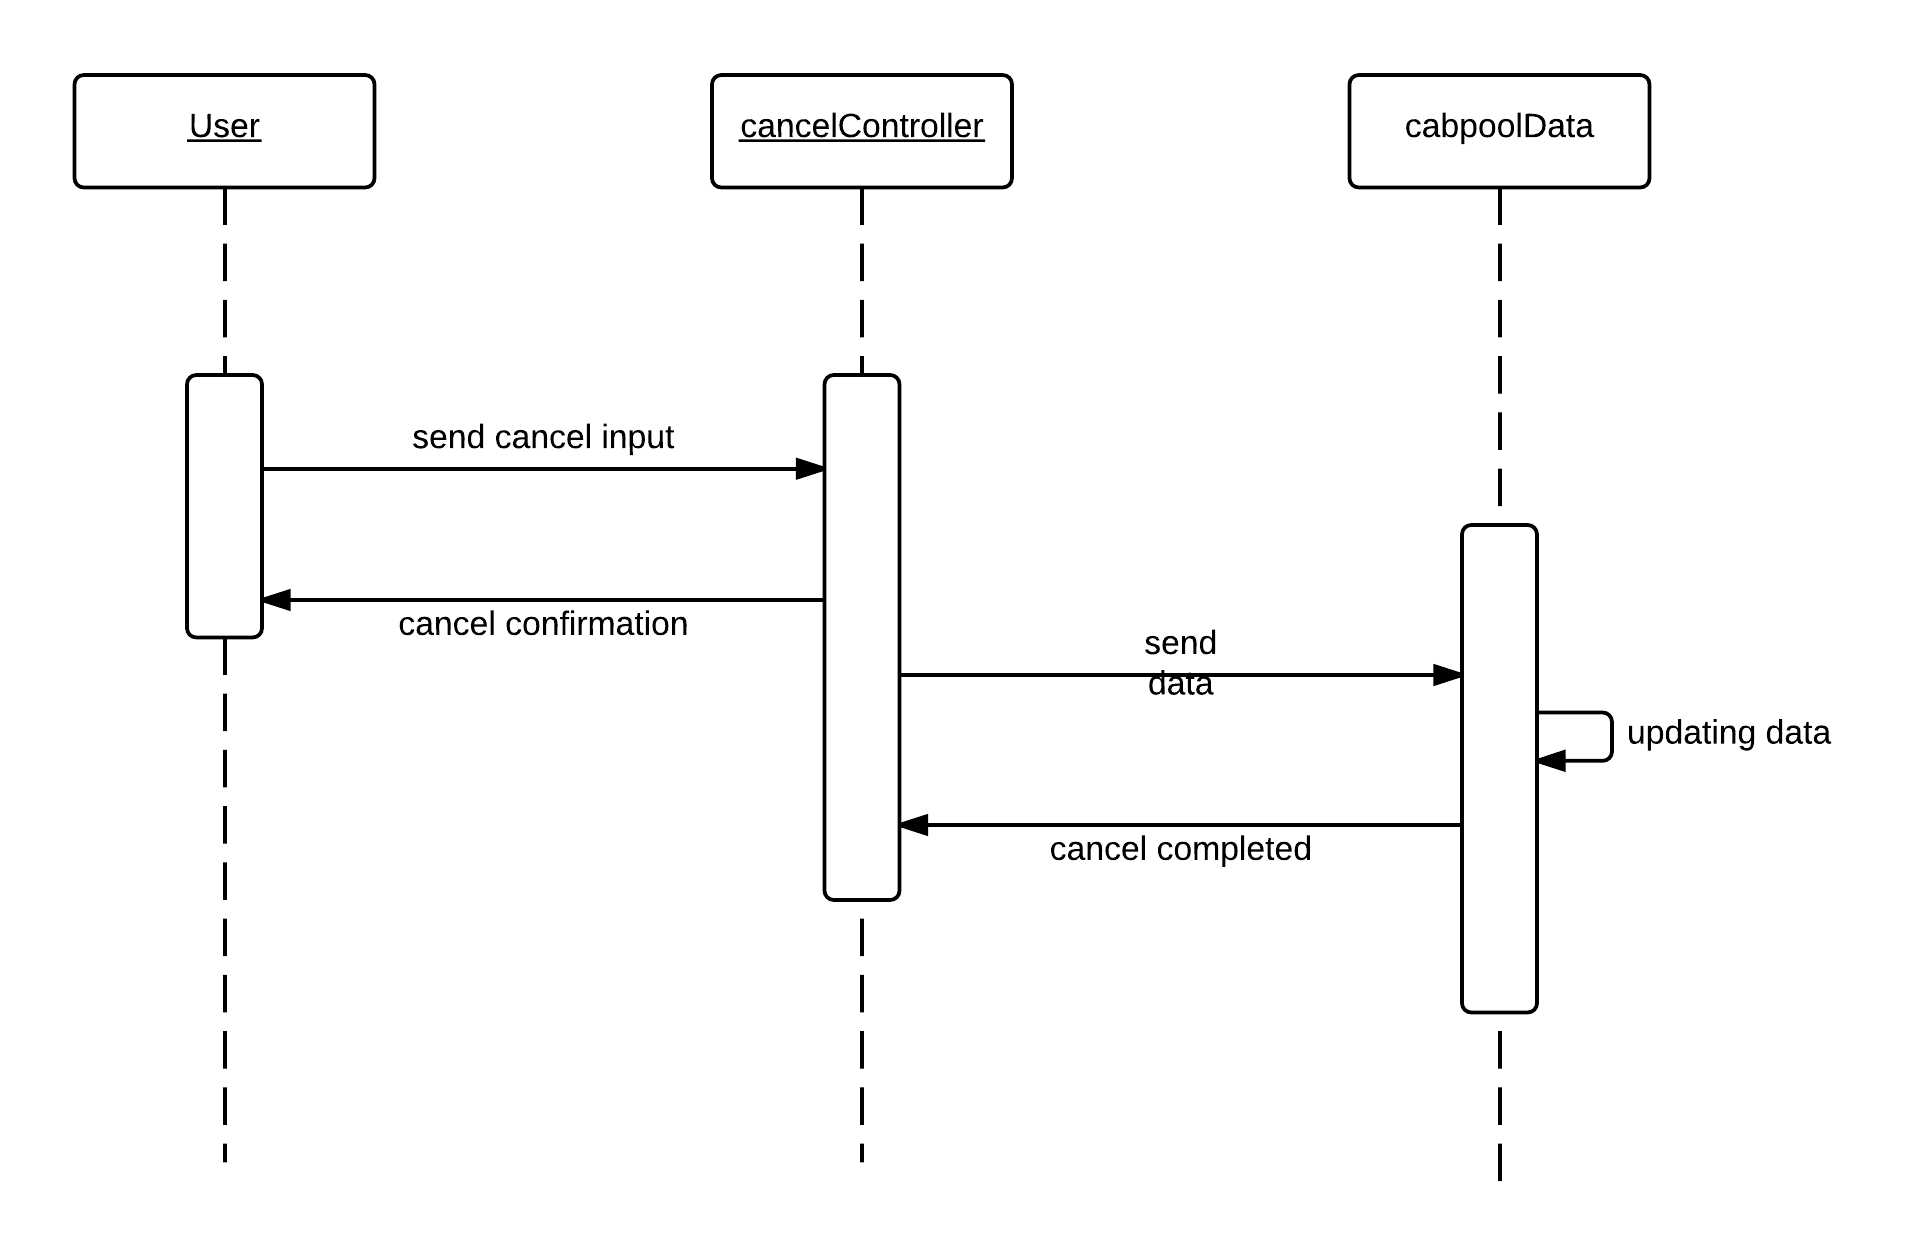
\includegraphics[width=1\textwidth]{CancelSequence.png}
	\caption{\textbf{Sequence Diagram of CancelSequence} How a user cancels a request for pickup.}
\end{figure}
% End Subsection

\subsection{LoginSequence}

\begin{figure}[H]
\label{logSeq}
	\centering
	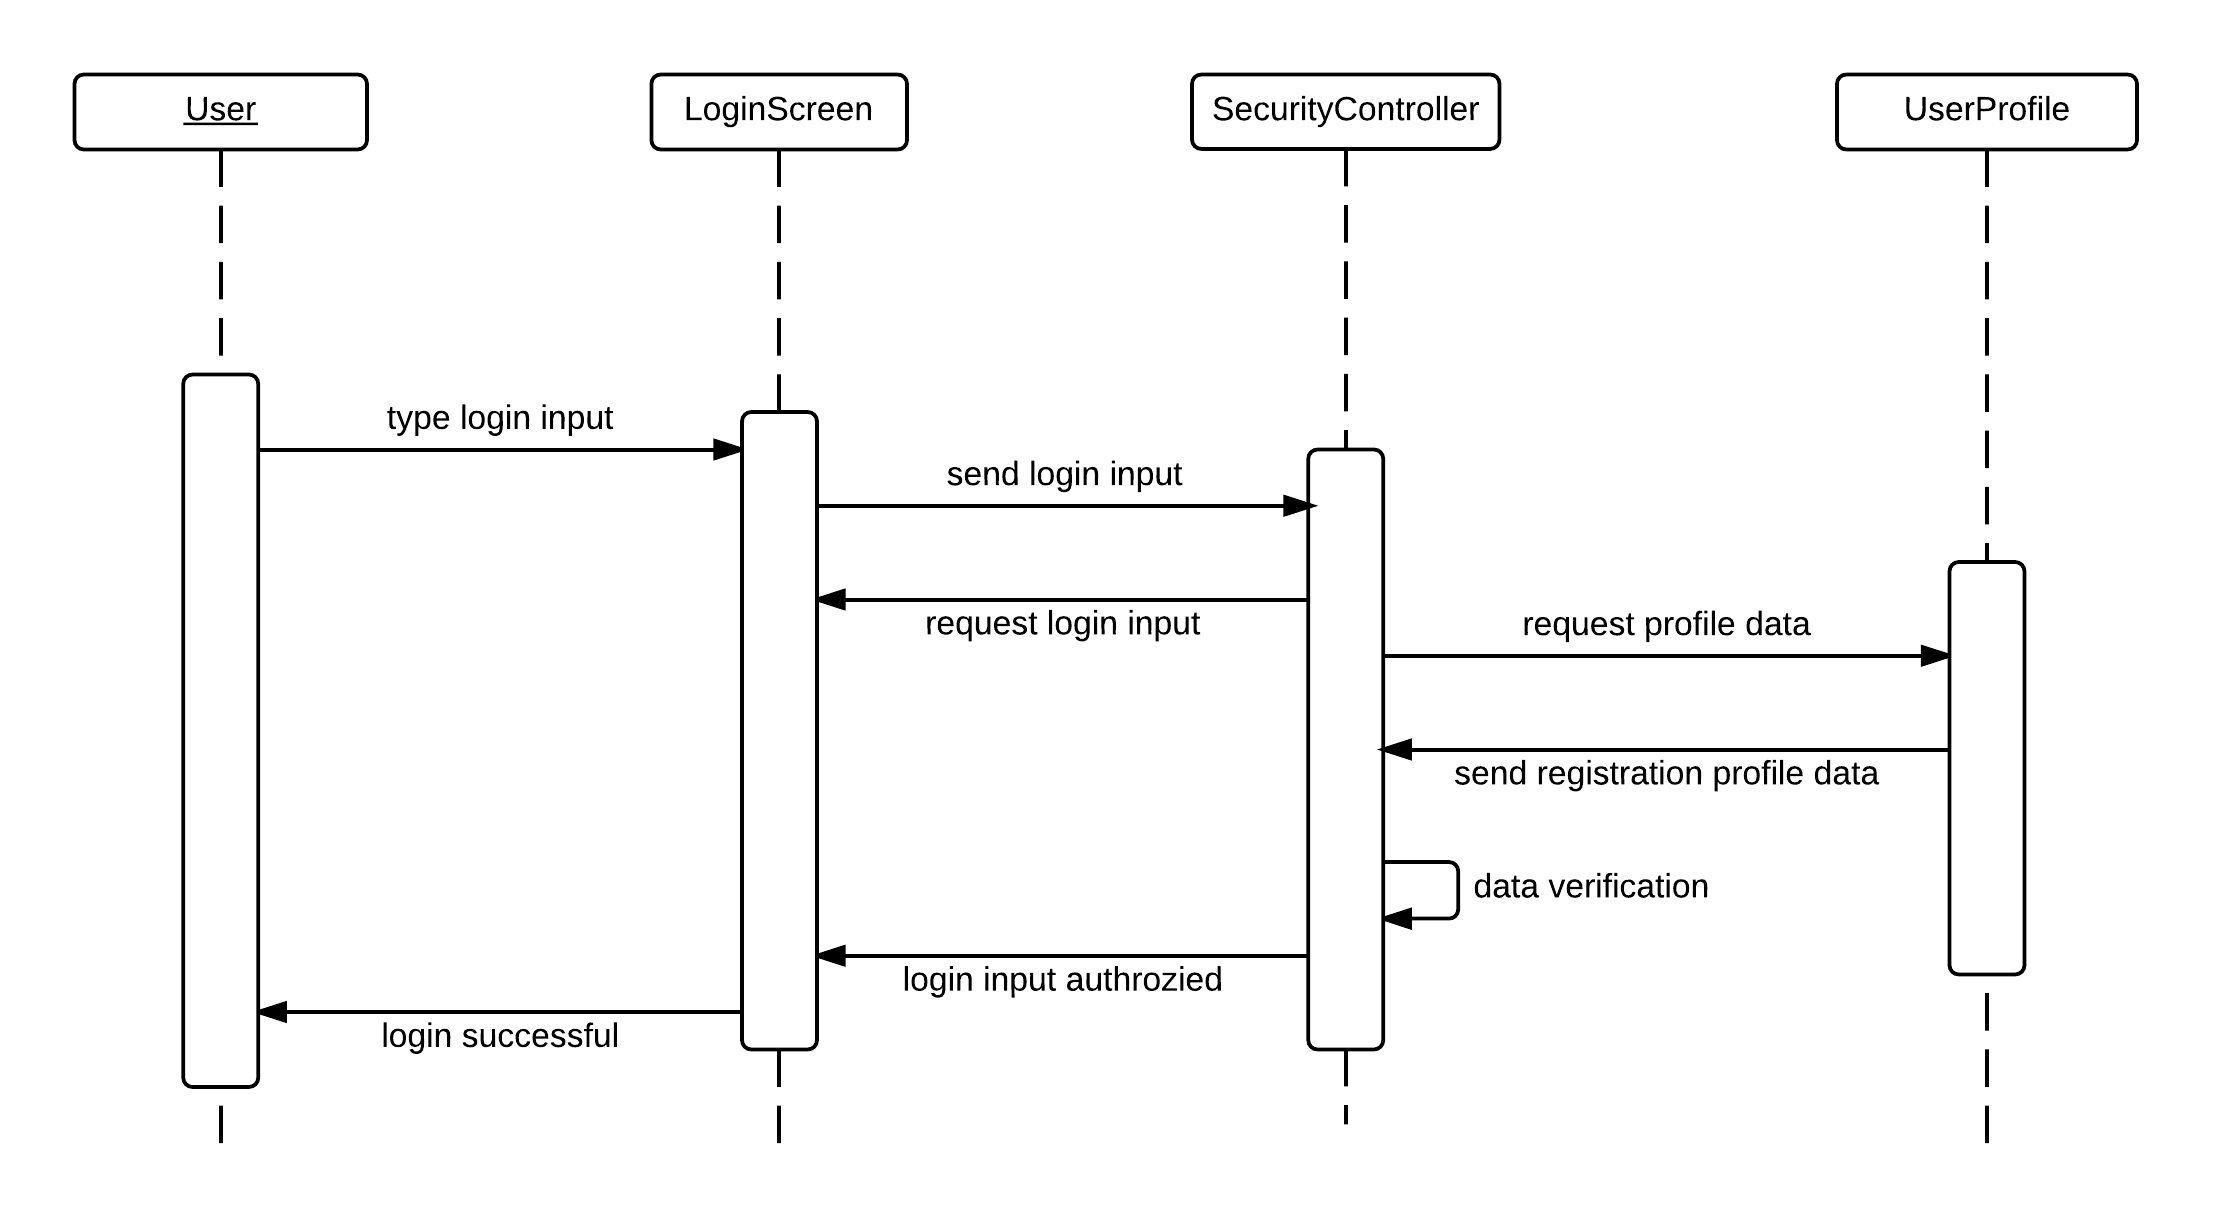
\includegraphics[width=1\textwidth]{LoginSequence.png}
	\caption{\textbf{Sequence Diagram of Login} The progression of the user logging in.}
\end{figure}
% End Subsection

\subsection{ModifyProfileSequence}

\begin{figure}[H]
\label{MPSeq}
	\centering
	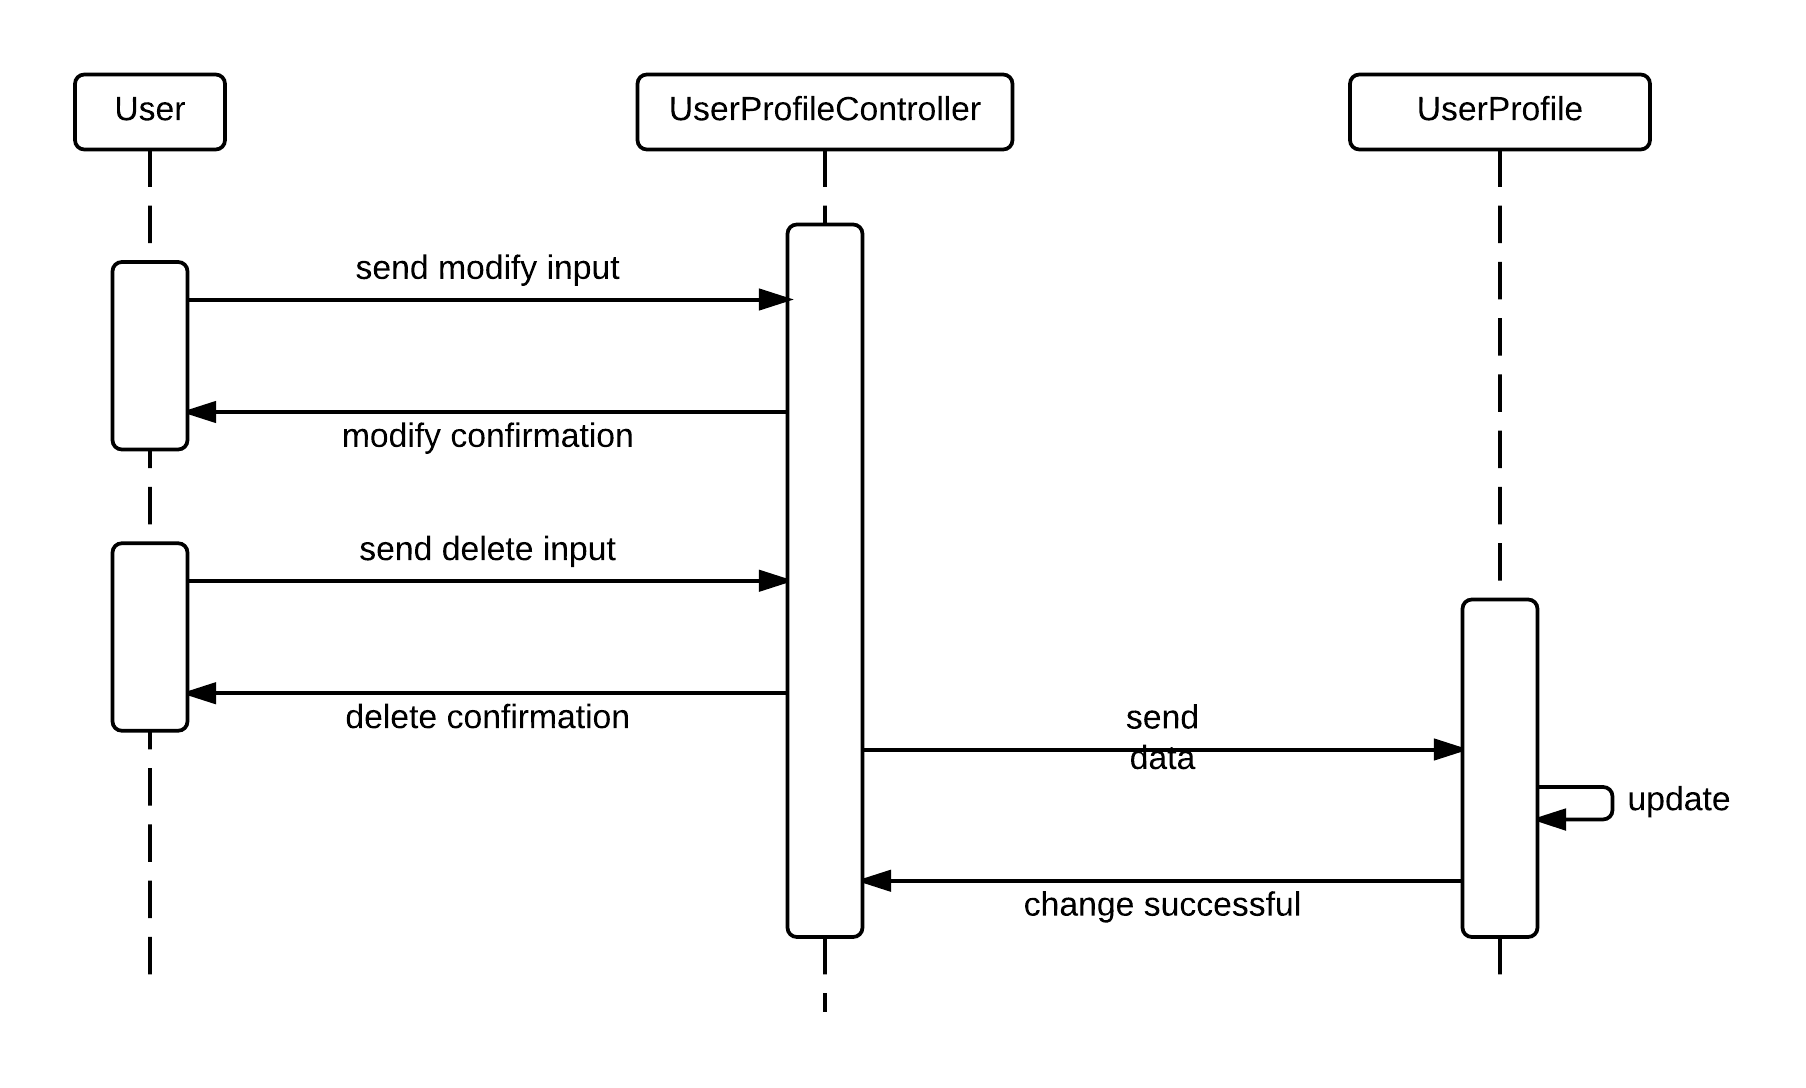
\includegraphics[width=1\textwidth]{ModifyProfileSequence.png}
	\caption{\textbf{Sequence Diagram of ModifyProfile} When the user modifies their profile details.}
\end{figure}
% End Subsection

\subsection{OfferSequence}

\begin{figure}[H]
\label{ofrSeq}
	\centering
	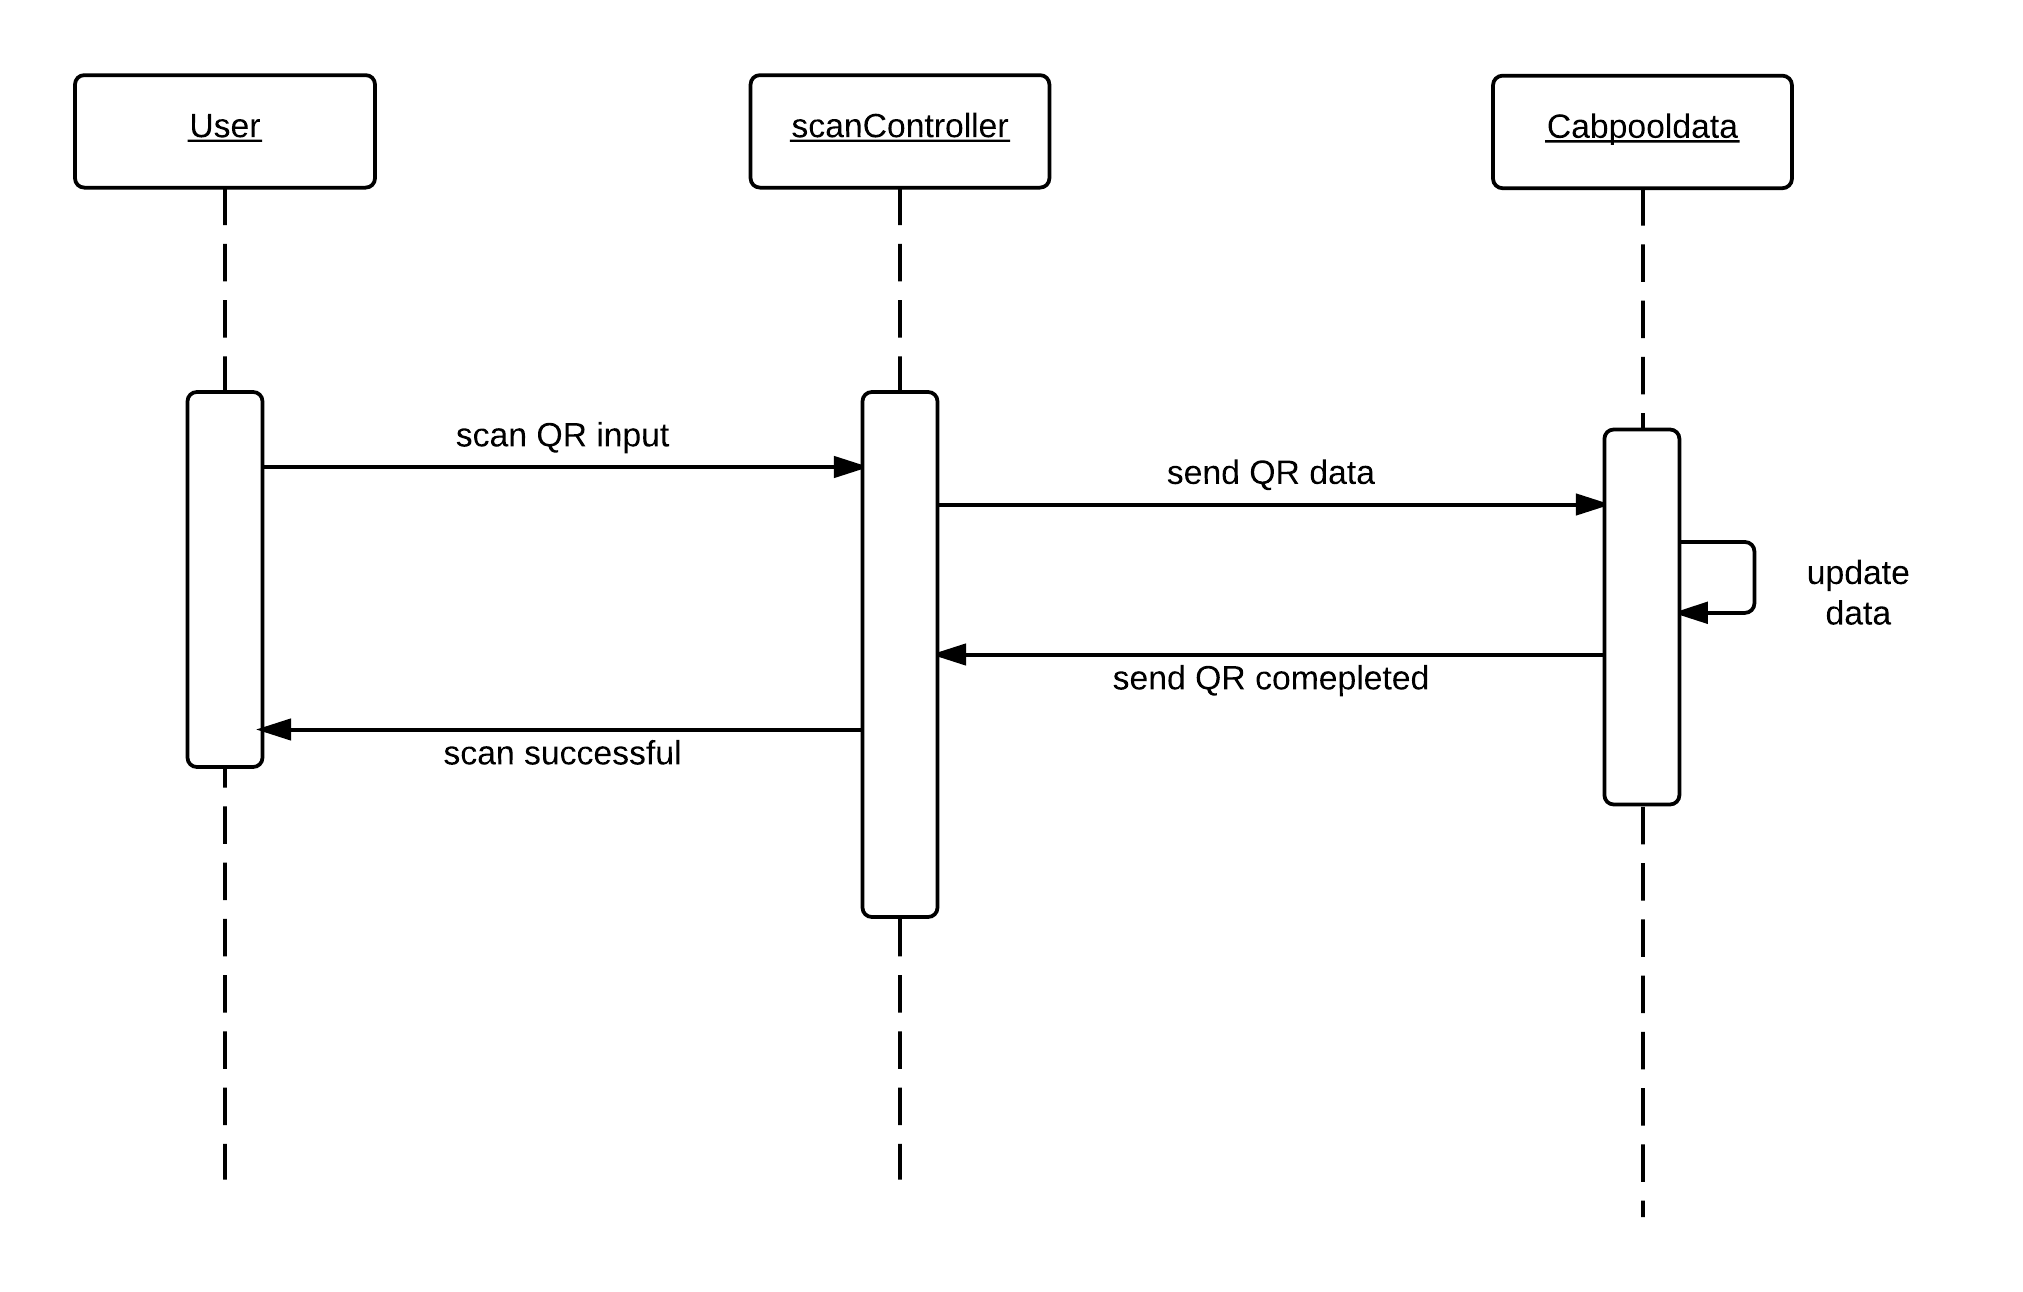
\includegraphics[width=1\textwidth]{OfferSequence.png}
	\caption{\textbf{Sequence Diagram of OfferSequence} When someone accepts an offer by scanning the QR code.}
\end{figure}
% End Subsection

\subsection{PaymentSequence}

\begin{figure}[H]
\label{paySeq}
	\centering
	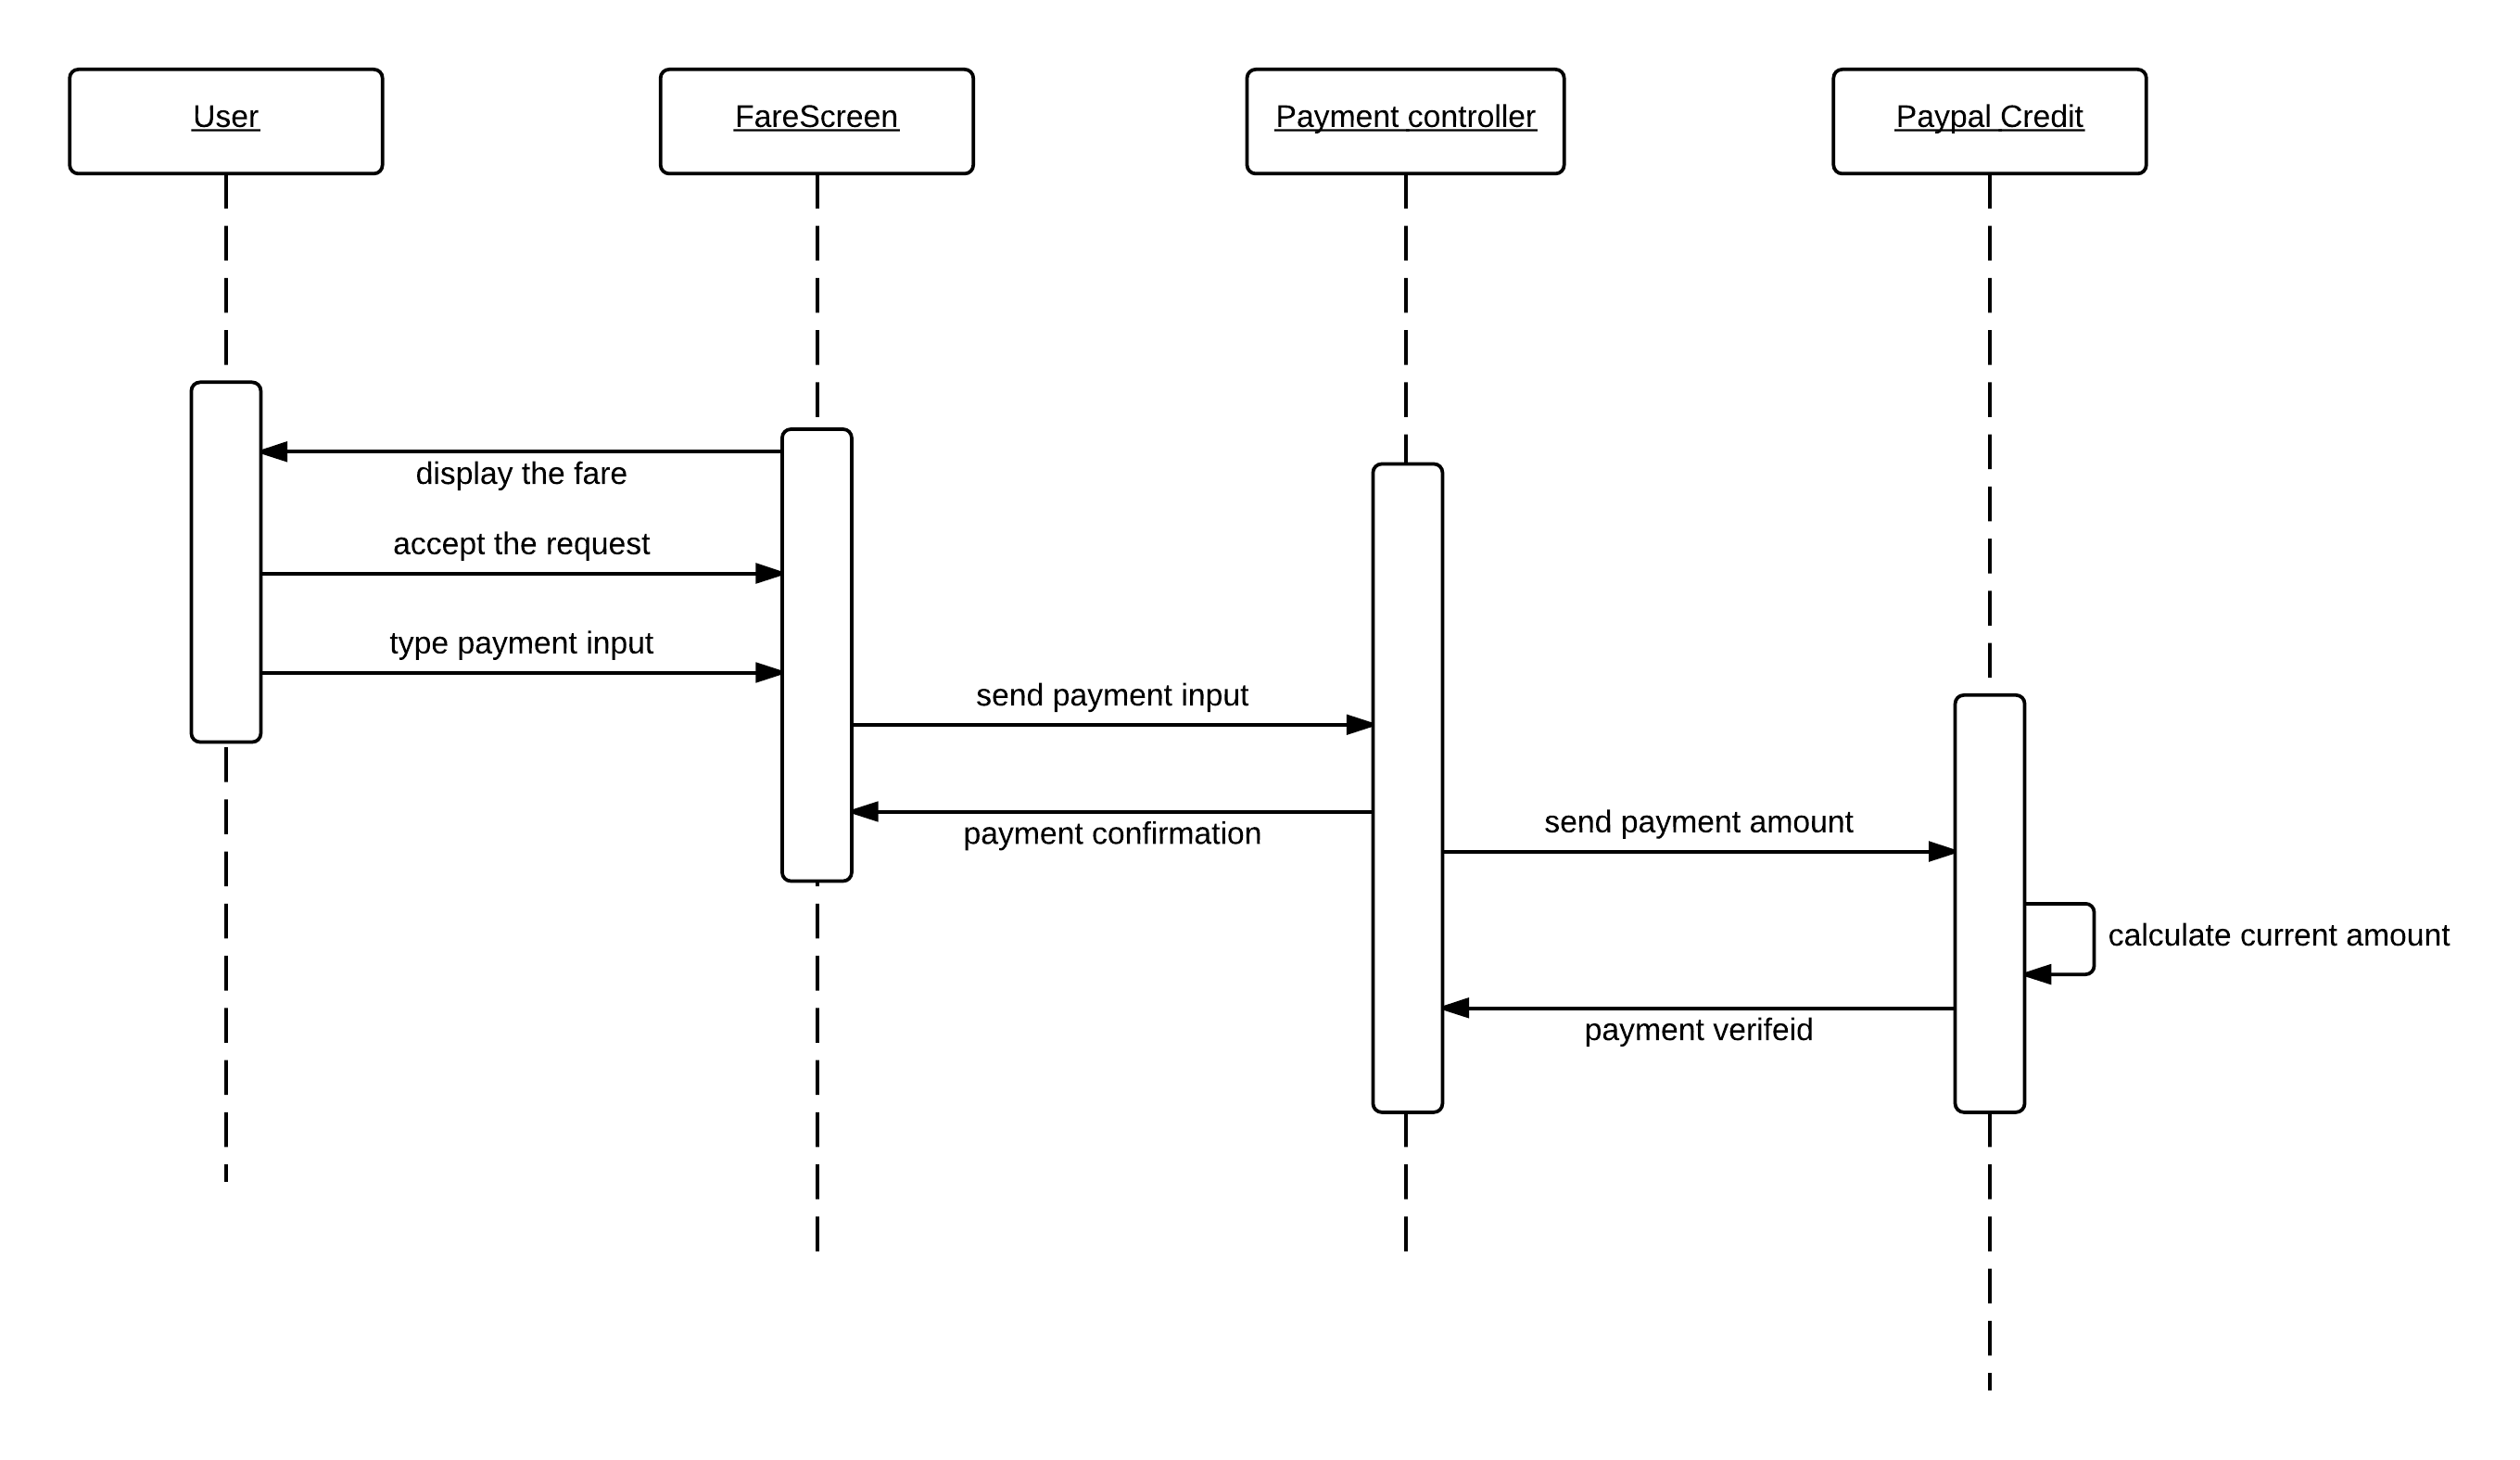
\includegraphics[width=1\textwidth]{PaymentSequence.png}
	\caption{\textbf{Sequence Diagram of PaymentSequence} When someone has finished their cab ride and it's time to pay, using PayPal.}
\end{figure}
% End Subsection

\subsection{RateSequence}

\begin{figure}[H]
\label{raSeq}
	\centering
	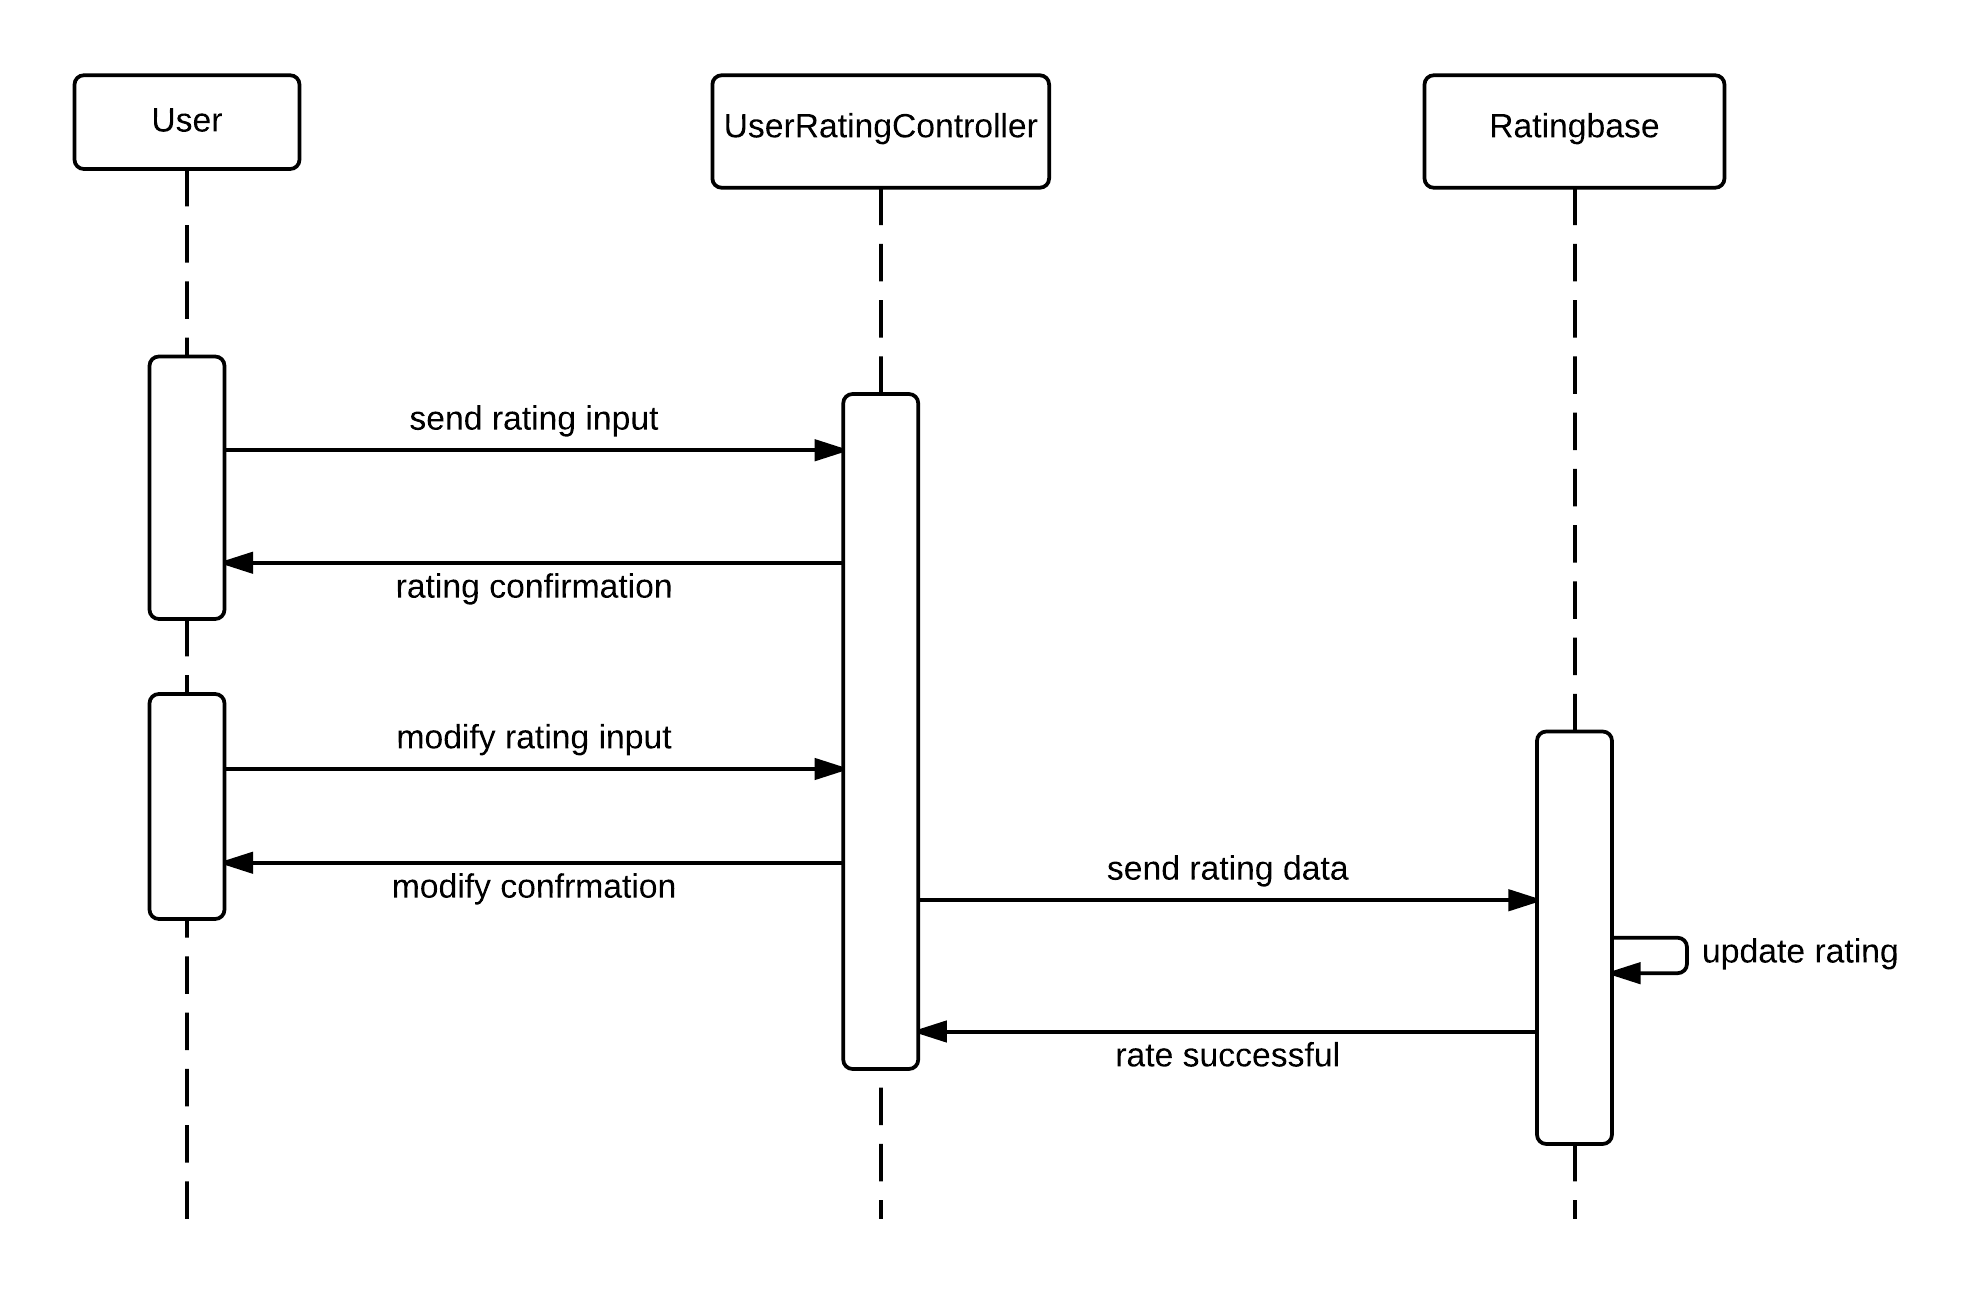
\includegraphics[width=1\textwidth]{RateSequence.png}
	\caption{\textbf{Sequence Diagram of RateSequence} When someone rates a fellow cab rider.}
\end{figure}
% End Subsection

\subsection{ReceiveSequence}

\begin{figure}[H]
\label{recSeq}
	\centering
	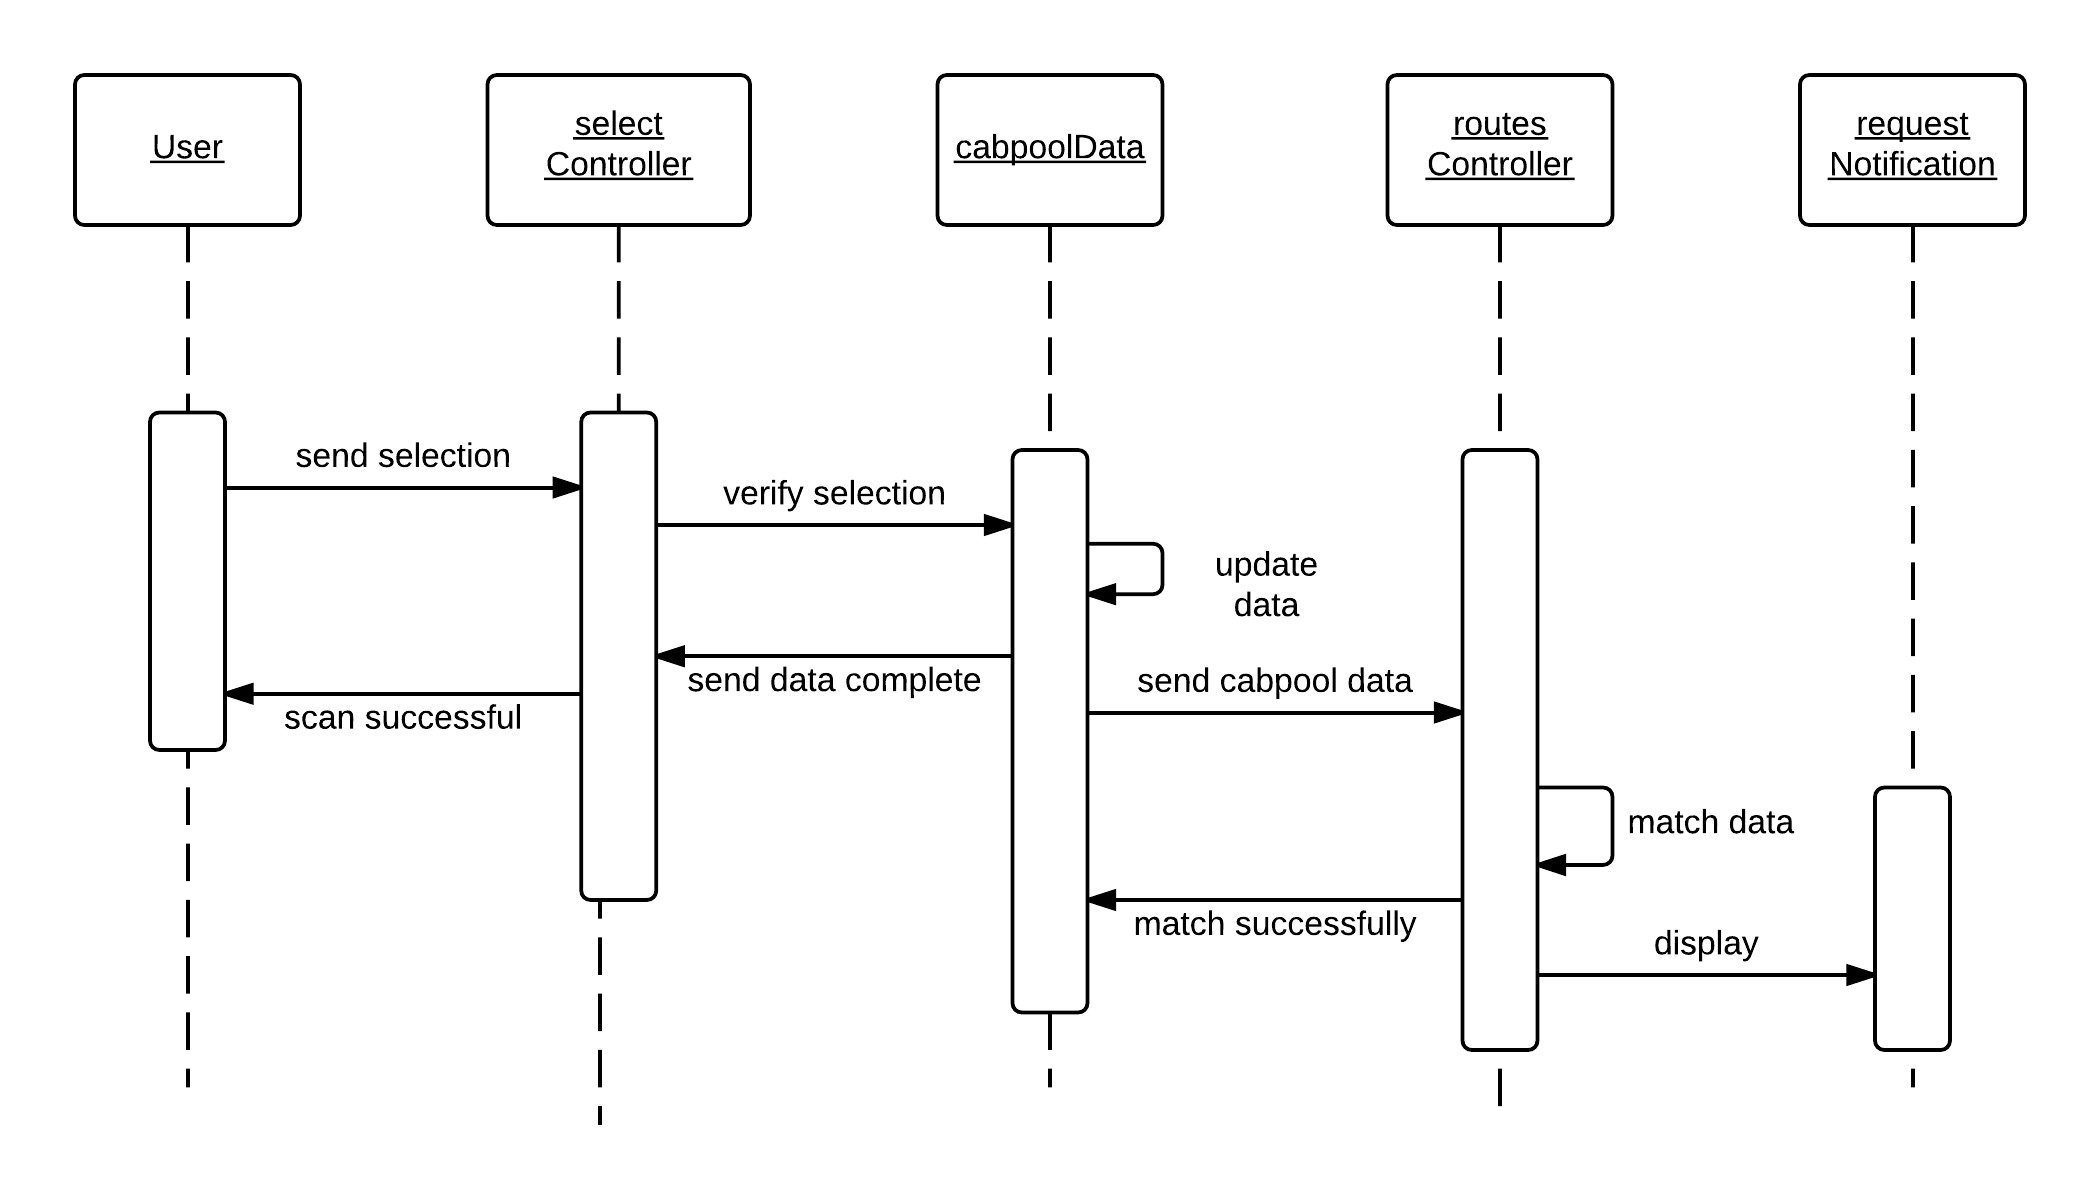
\includegraphics[width=1\textwidth]{ReceiveSequence.png}
	\caption{\textbf{Sequence Diagram of ReceiveSequence} When a user chooses a cabpool to join.}
\end{figure}
% End Subsection

\subsection{RegistrationSequence}

\begin{figure}[H]
\label{regSeq}
	\centering
	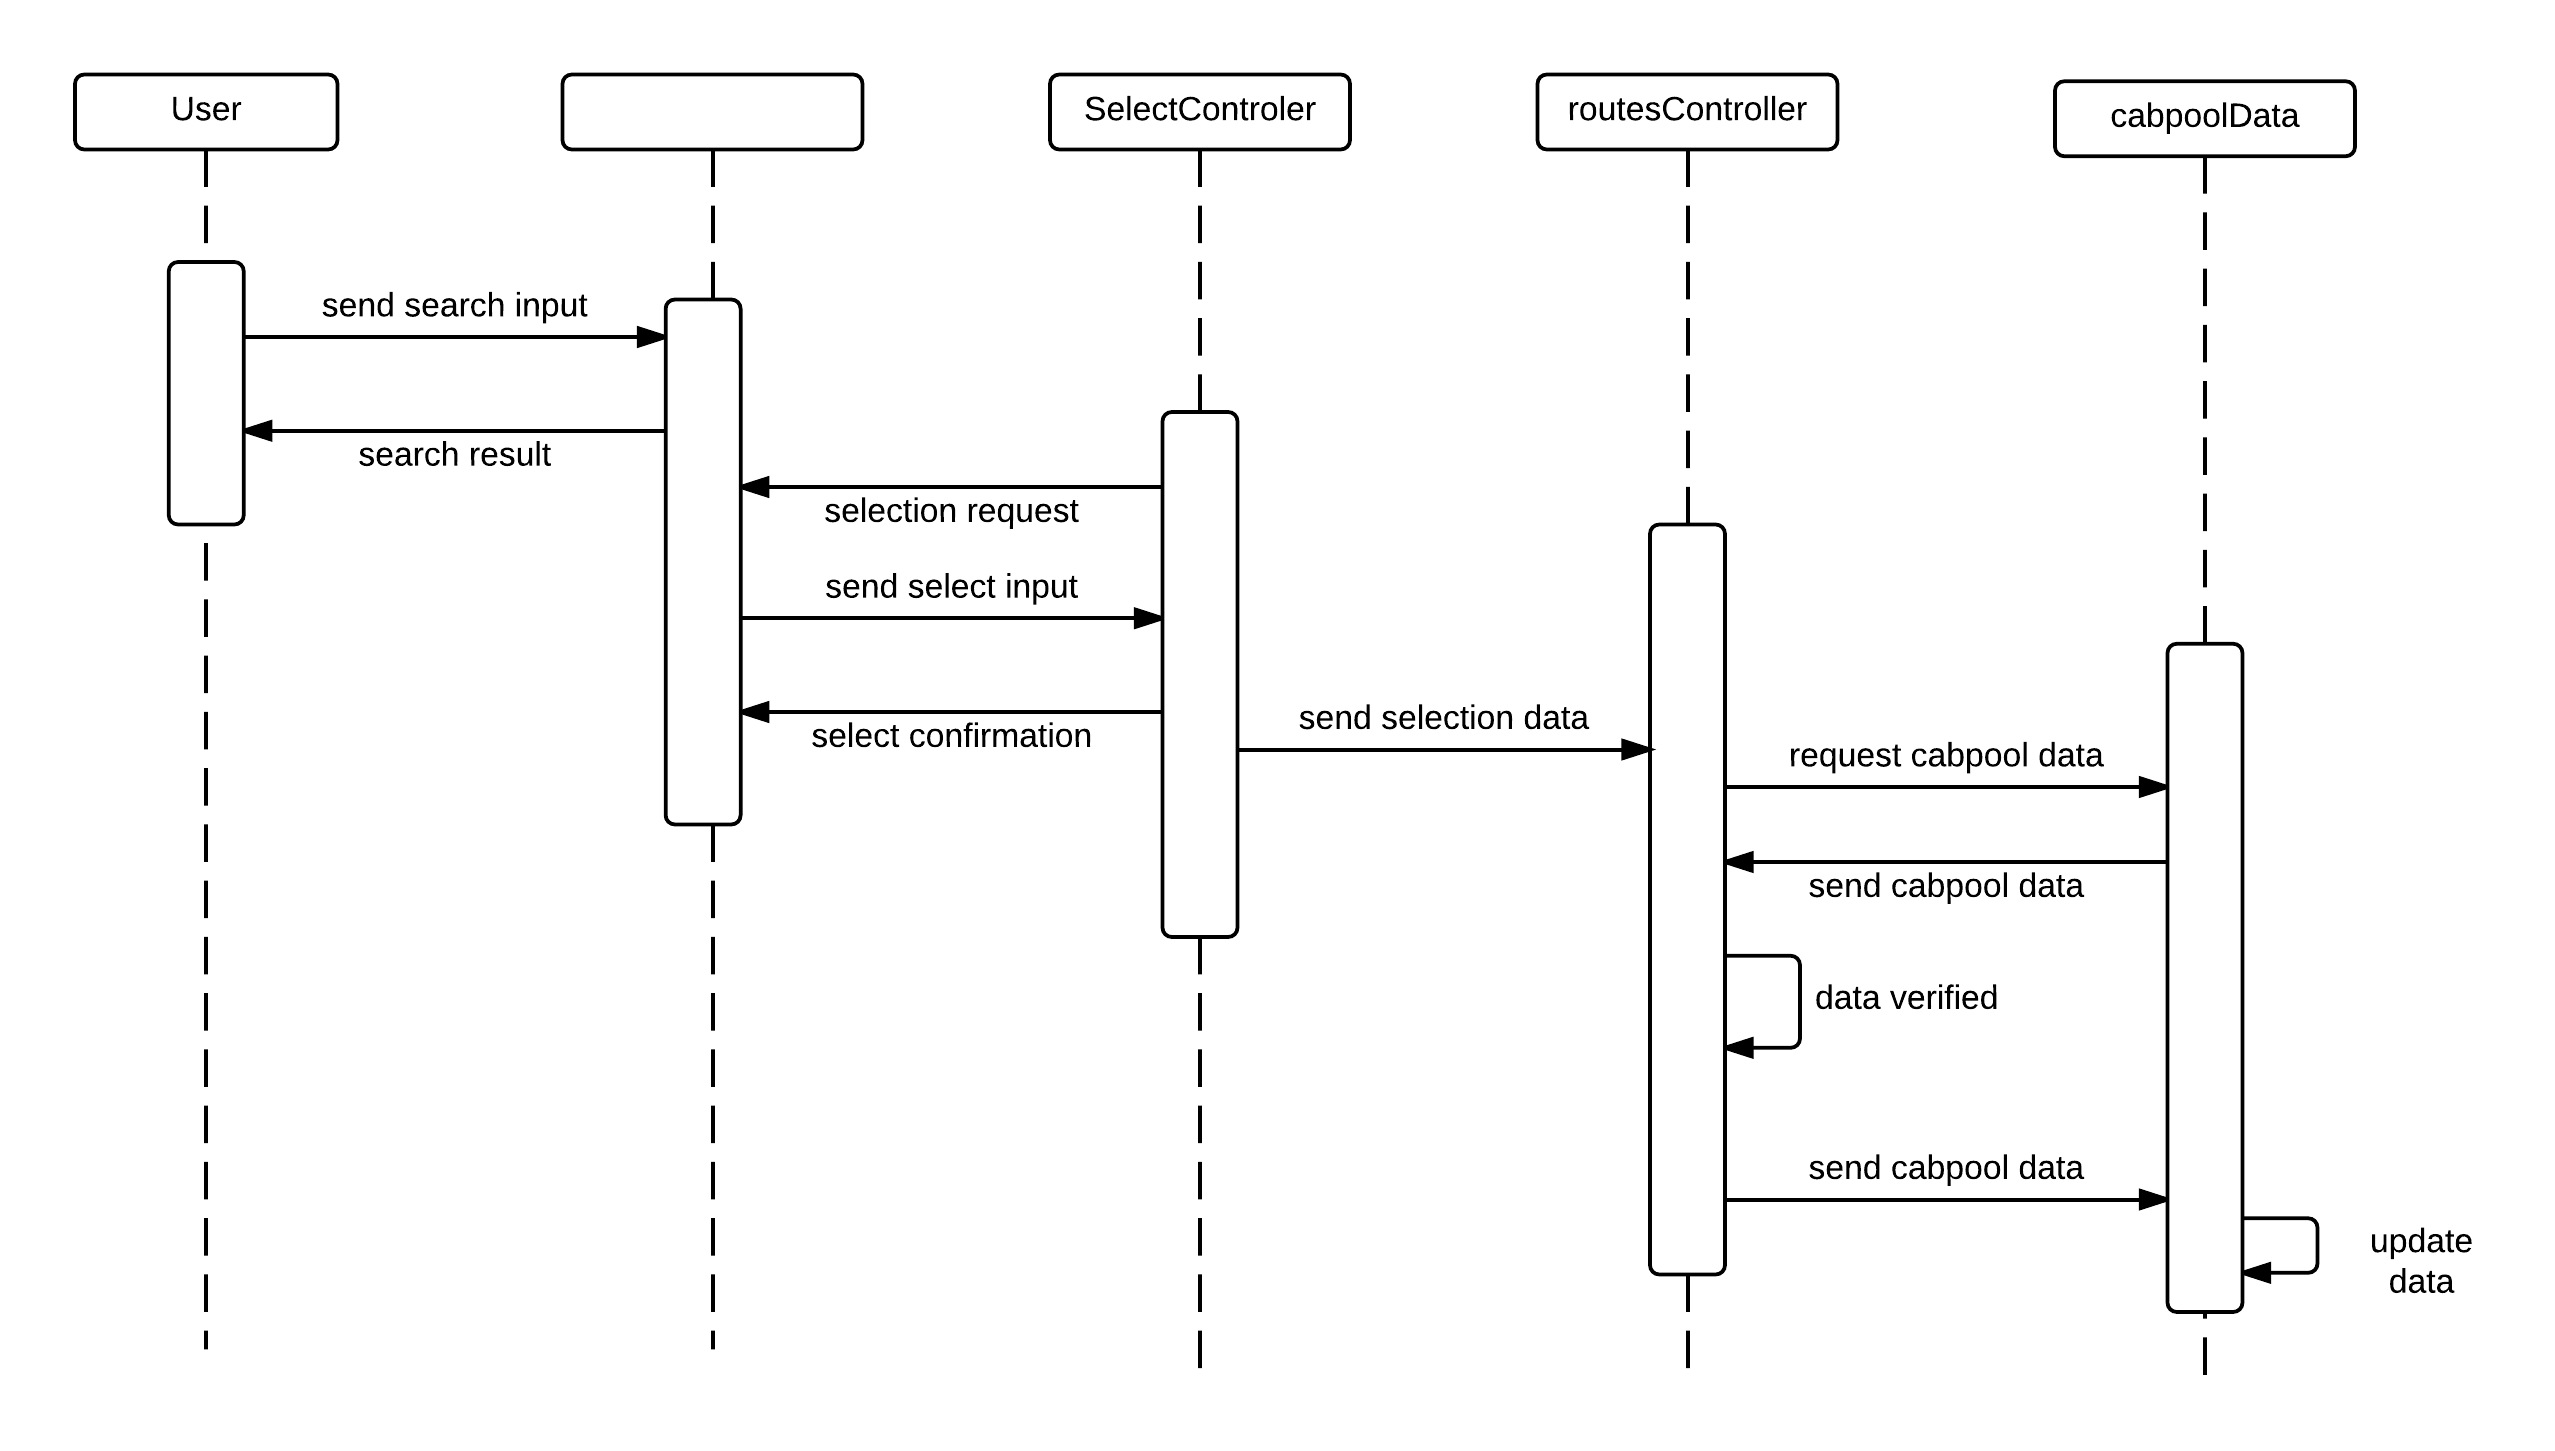
\includegraphics[width=1\textwidth]{RequestSequence.png}
	\caption{\textbf{Sequence Diagram of RegestrationSequence} When the user is first creating a profile.}
\end{figure}
% End Subsection

\subsection{RequestSequence}

\begin{figure}[H]
\label{reqSeq}
	\centering
	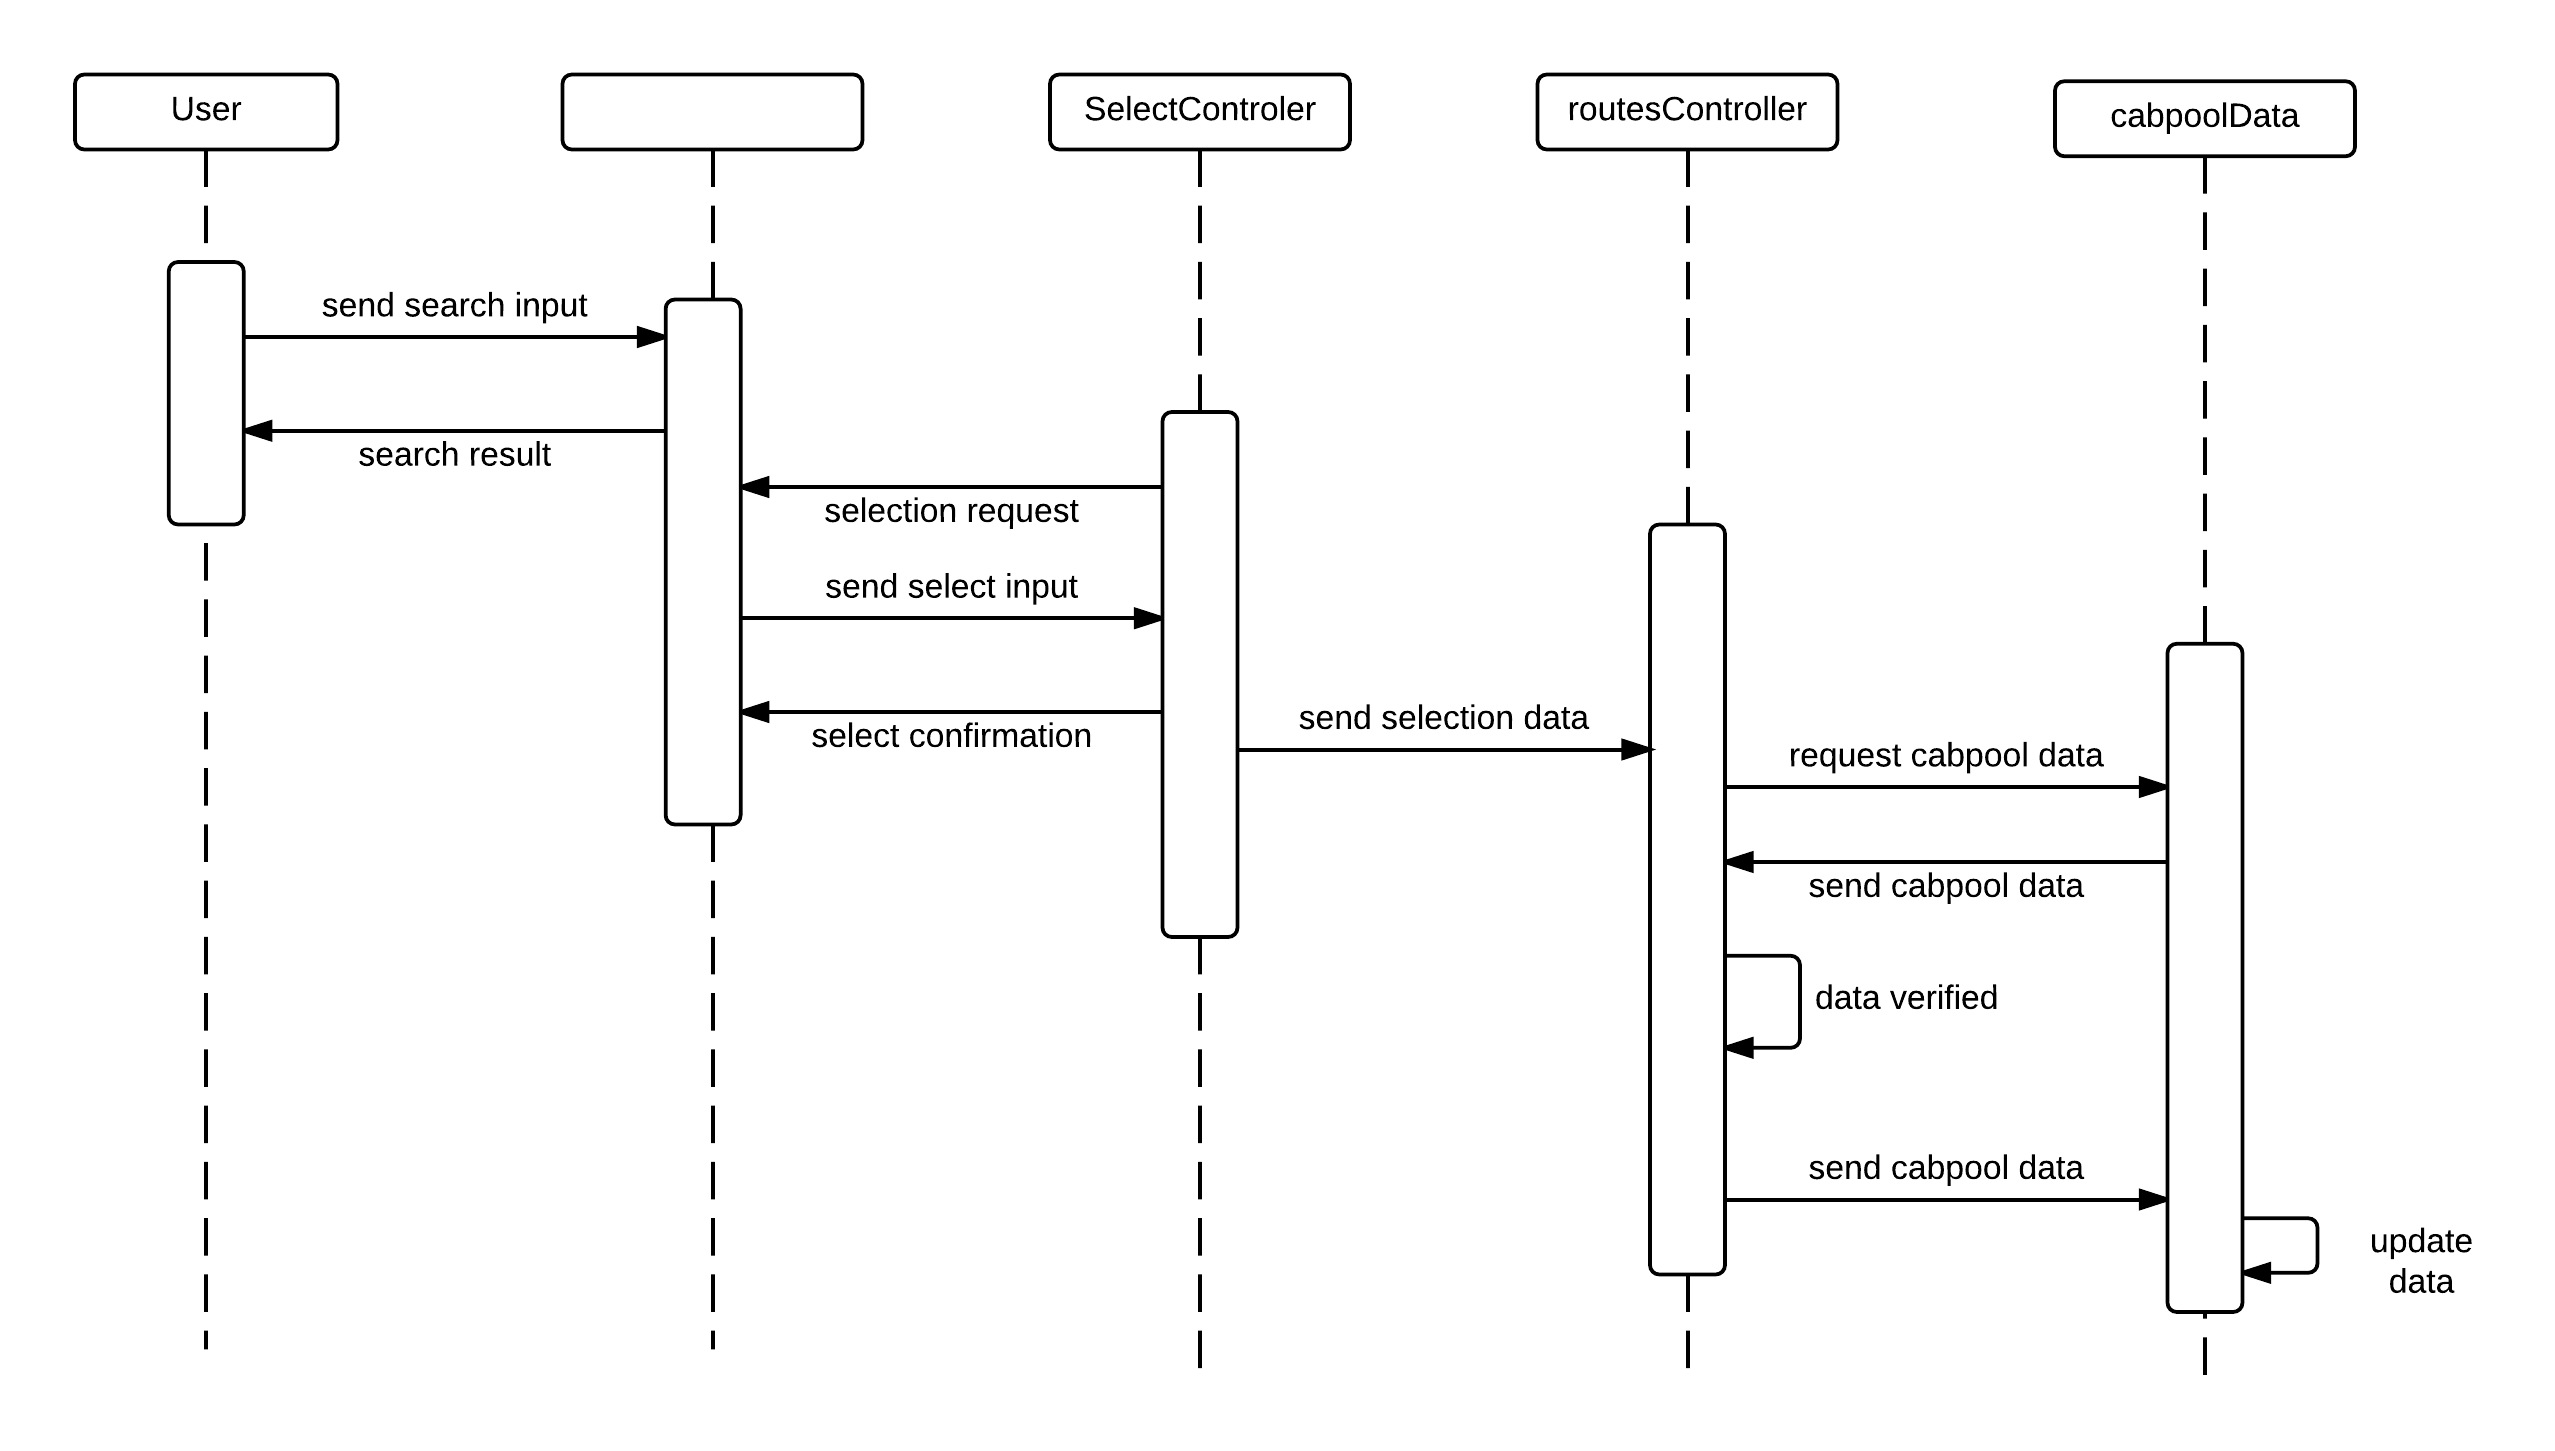
\includegraphics[width=1\textwidth]{RequestSequence.png}
	\caption{\textbf{Sequence Diagram of RequestSequence} When a user requests a cabpool.}
\end{figure}
% End Subsection
% End Section


% Begin Section
\section{Detailed Class Diagram}
\label{DetailedClass}

\begin{figure}[H]
\label{classDig}
	\centering
	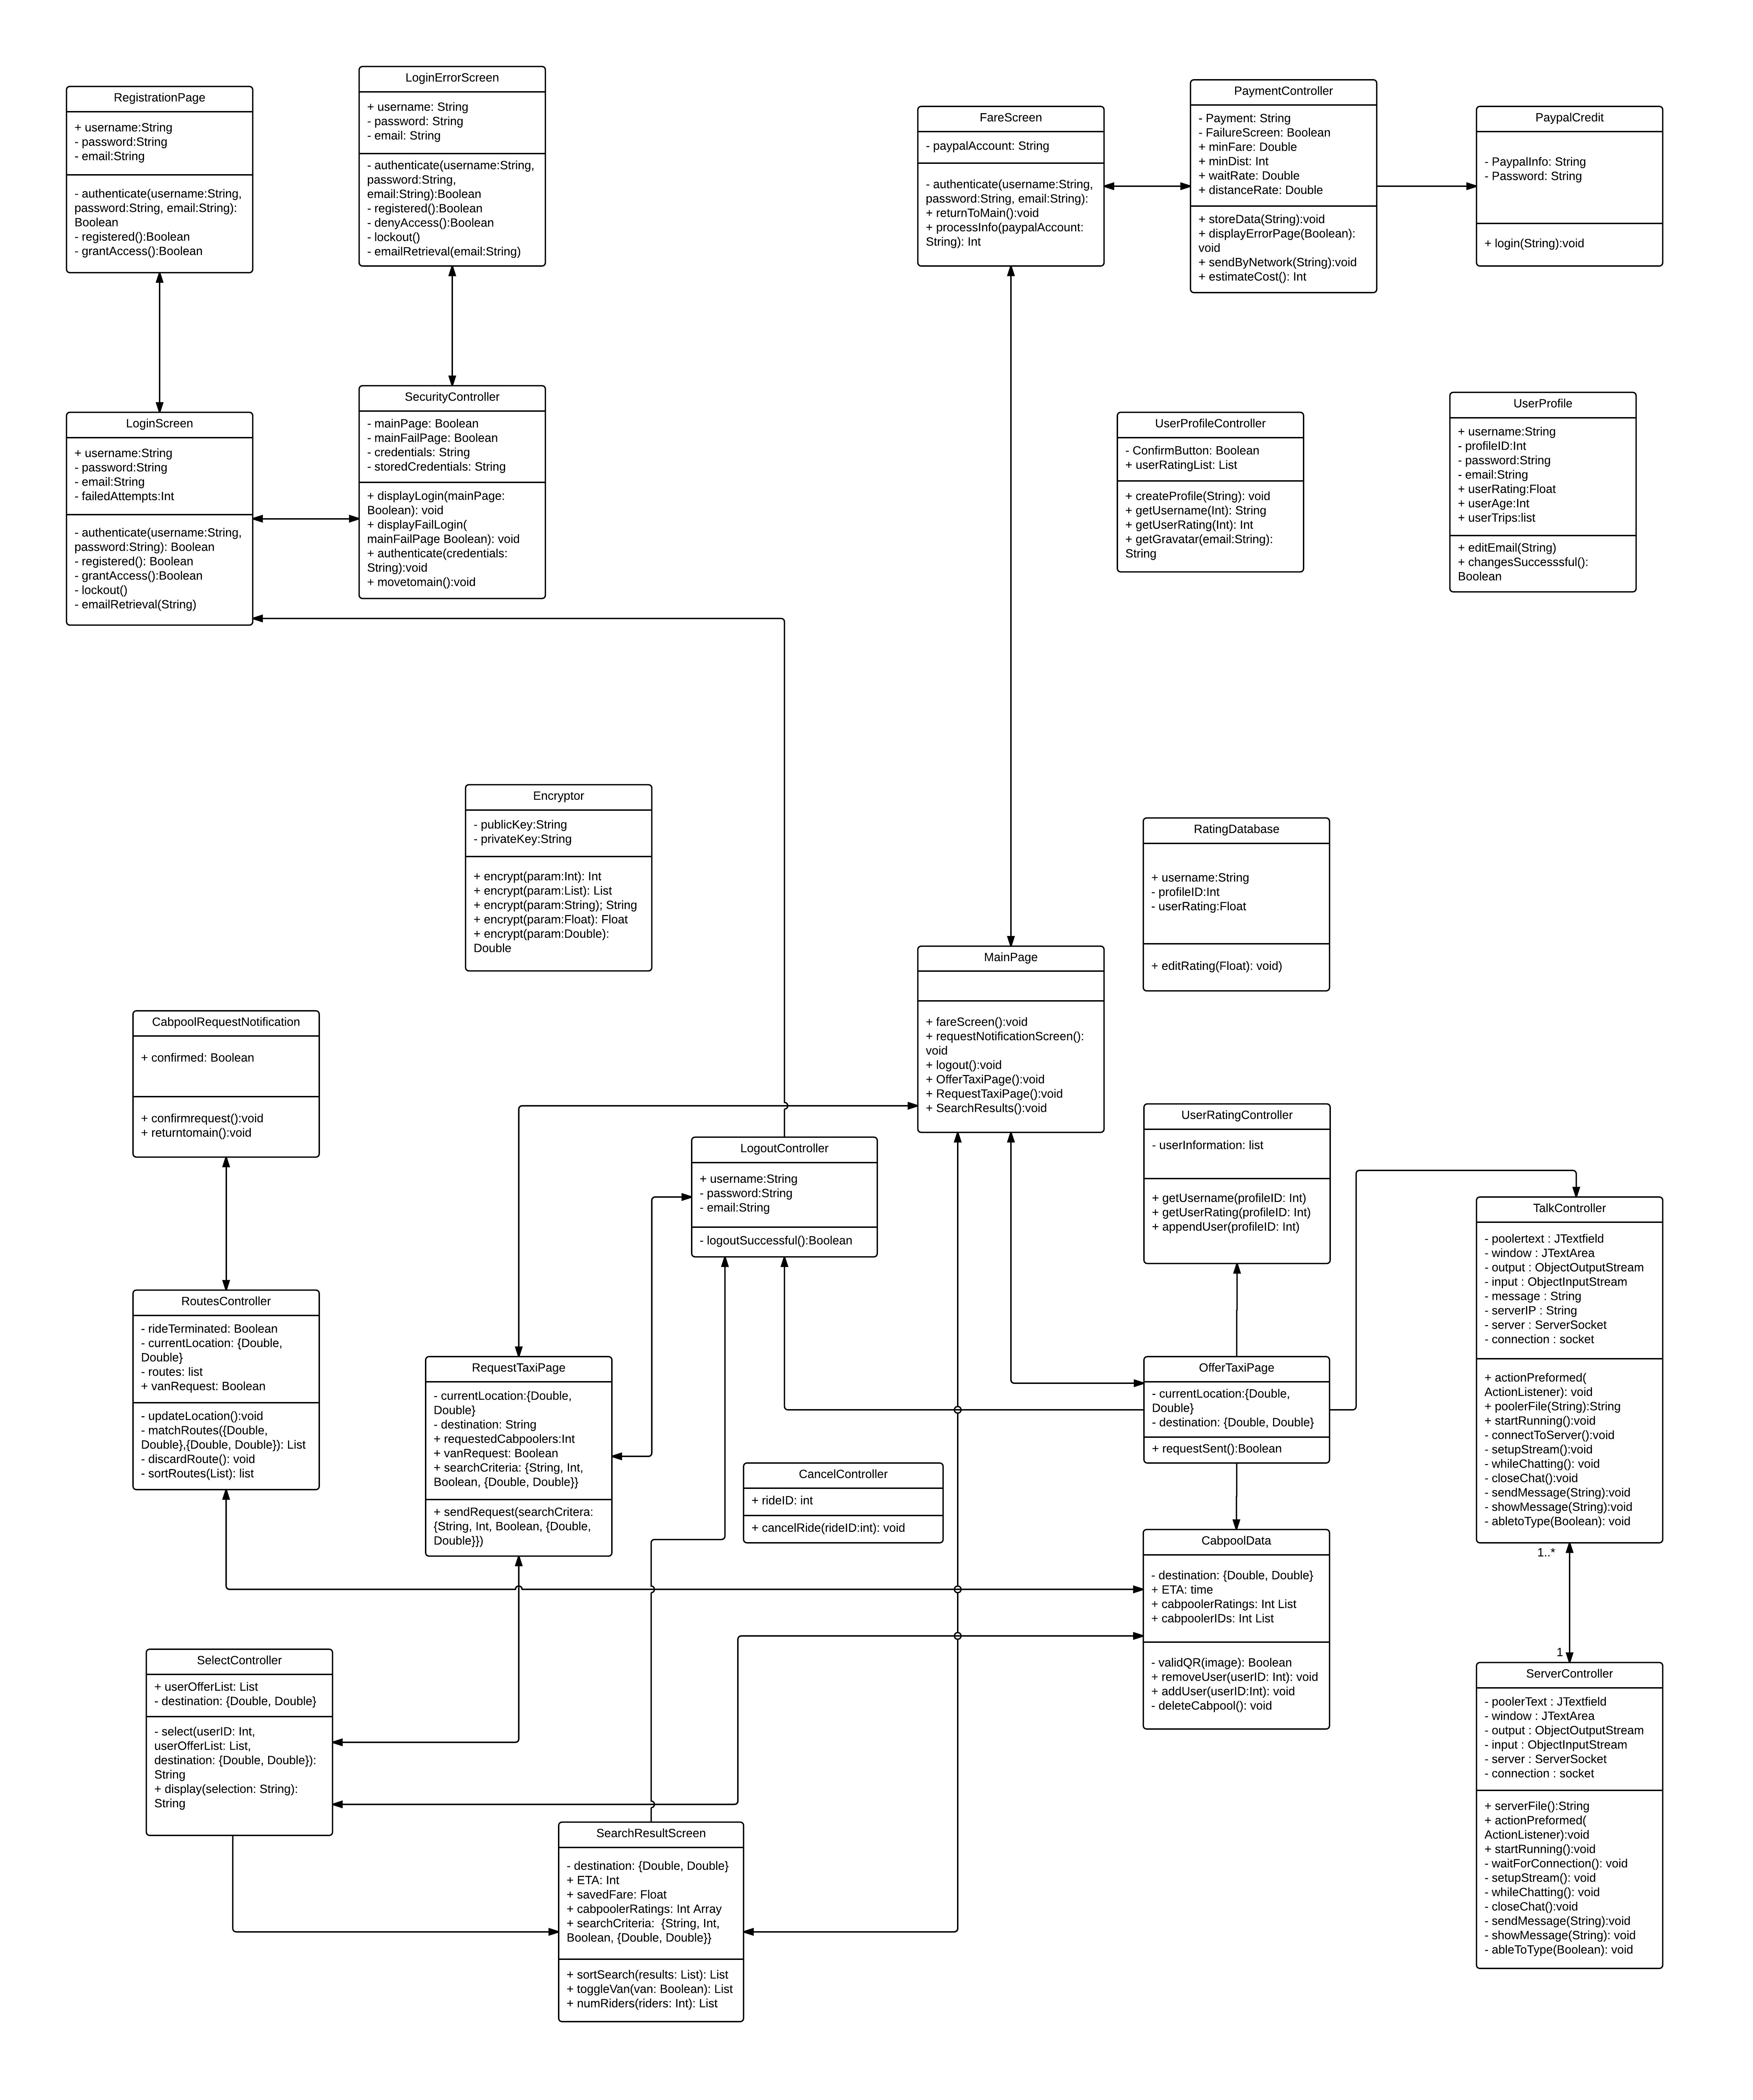
\includegraphics[width=1\textwidth]{class.png}
	\caption{\textbf{Detailed Class Diagram} Classes and their relationships between each other are outlined in this document.}
\end{figure}
% End Section

\section{Cake}
\begin{figure} [H]
    \centering
    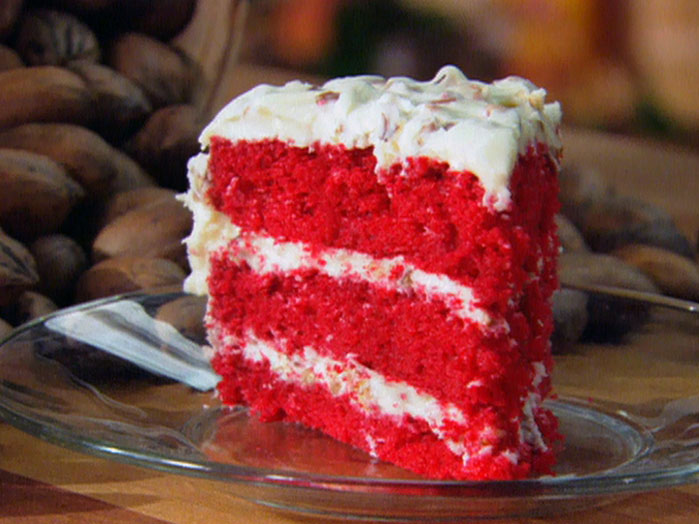
\includegraphics[width=0.48\textwidth]{cake.jpg}
	\caption{\textbf{Cake} Red velvet cake for your time.}
\end{figure}

\appendix
\section{Division of Labour}
\label{DoL}
% Begin Section
Include a Division of Labour sheet which indicates the contributions of each team member. This sheet must be signed by all team members.

\begin{itemize}
    \item Kemal \textsc{Ahmed}:
        \begin{itemize}
        \item Formatted this \LaTeX \ document
        \item Reviewed all controller state diagrams before putting the picture in the \LaTeX \ document
        \item \hyperref[LCState]{LogoutController State diagram}
        \item Learned and taught encryption protocols to group
        \item Fed the group at meetings
        \item Class Diagram
        \end{itemize}
    \item Mitchell \textsc{Spector}:
        \begin{itemize}
        \item Chat functionality
        \item Class Diagram
        \end{itemize}
    \item Sahajmeet \textsc{Bhutta}:
        \begin{itemize}
        \item Introduction
        \item Helped all other members with corrections in diagrams formatting and correctness of information
        \item Class Diagram
        \end{itemize}
    \item Xue \textsc{Lin}
        \begin{itemize}
        \item Sequence Diagrams
        \end{itemize}
    \item Yuchen \textsc{Xiao}
        \begin{itemize}
        \item Encryptor
        \item \hyperref[SeqDi]{Cancel Sequence Diagram}
        \item UserProfileController
        \end{itemize}
\end{itemize}

% End Section

\end{document}
%------------------------------------------------------------------------------